% BD: chapter skeleton for Assignment 7 (course Chapter 5), to become devopsSre.tex in the Gitea manual repo
% and be included in devopsITManual.tex after devopsJenkins. Section labels are fixed here so that
% SD's and BD's regions can cite each other with \SectionRef{...} from the start.
% Owners: SD = rows 1, 2, 3, 5; BD = rows 4, 6, 7, 8. Points per rubric 5.5: 15, 15, 10, 15, 10, 15, 10, 10.
\chapter{Monitoring and reliability (SRE)}
\ChapterLabel{Sre}
\index{monitoring}\index{SRE}

% --- Short overview (BD, written last): what was added to the server, one paragraph, link to the successful PDF build and the reviewed final commit.

% ===== SD region: rows 1, 2, 3 =====
% Region: sreDeployment (single owner; edit only your own region)
\section{Deployment and capacity (15 points)}\label{Section:sreDeployment}
\textbf{Owner:} SD. \textbf{Status:} deployed November 10, 2026; restart test November 11, 2026 \StatusPass.

\paragraph{Baseline and capacity.} Before anything was added, the server was read without changes (\ListRef{110}):
an EC2 \texttt{t3.micro} with 913~MiB of RAM, of which only 200~MiB was available and 425~MiB was already in swap, while
Gitea, Jenkins, Caddy and the Actions runner were running. Four more containers would not have fit. BD decided to resize
the same instance to \texttt{t3.small} (same disk and Elastic IP); afterwards the host had 1,909~MiB with 1,064~MiB
available and no swap in use (\ListRef{140}). The root disk had 8.4~GB free, enough for the images (about 1.4~GB) and
Prometheus' capped storage.

\paragraph{What runs.} Four separate containers, all from images published by the projects themselves; nothing is built
locally and no Dockerfile is written. Tags are pinned to exact releases (never \texttt{latest}) and the pulled image
digests are recorded (\ListRef{111} for the choice, \ListRef{112} for the digests on the server).

\begin{tabularx}{\linewidth}{L{2.9cm}L{4.6cm}Y}
\caption{Monitoring containers, versions, and limits\label{Table:SreContainers}}\\
\toprule \textbf{Container} & \textbf{Image} & \textbf{Role, limit, storage}\\ \midrule
\endfirsthead
\toprule \textbf{Container} & \textbf{Image} & \textbf{Role, limit, storage}\\ \midrule
\endhead \bottomrule \endlastfoot
\texttt{prometheus} & \texttt{prom/prometheus:}\newline\texttt{v3.16.0} & scrapes every 30\,s and stores metrics; 256~MiB; volume \texttt{monitoring\_prometheus\_data}, kept 7 days or 1~GB, whichever comes first\\
\texttt{grafana} & \texttt{grafana/grafana:}\newline\texttt{13.3.1} & dashboard and alerts; 384~MiB; volume \texttt{monitoring\_grafana\_data} (users, data source, dashboard, alert rules)\\
\texttt{node-exporter} & \texttt{quay.io/prometheus/}\newline\texttt{node-exporter:v1.12.1} & whole-host CPU, memory, root filesystem; 64~MiB; host \texttt{/} mounted read-only\\
\texttt{blackbox-}\newline\texttt{exporter} & \texttt{quay.io/prometheus/}\newline\texttt{blackbox-exporter:v0.29.1} & HTTPS probes of the Gitea and Jenkins login pages; 64~MiB; no storage\\
\end{tabularx}

The memory limits make sure that, if memory runs out, a monitoring container is stopped rather than Gitea or Jenkins.
Grafana's limit started at 256~MiB, but Grafana used 216~MiB while idle, so it was raised to 384~MiB on the first day
(recorded in \ListRef{112}). Retention of 7 days follows the course's lab suggestion; the 1~GB cap protects the root
disk that Jenkins builds also use.

\paragraph{Configuration in Gitea.} The non-secret files are in the \texttt{infra} repository, folder
\href{\GiteaURL/group1-startup/infra/src/branch/main/monitoring}{\texttt{monitoring}}, added through
\href{\GiteaURL/group1-startup/infra/issues/1}{issue \#1} and
\href{\GiteaURL/group1-startup/infra/pulls/2}{pull request \#2}. BD checked the Caddy block against the live
Caddyfile and the memory limits against the running containers, and merged it on November 11, 2026, 19:42~EST, as
merge commit \href{\GiteaURL/group1-startup/infra/commit/c03fb1b10e003554374404b7759cefa408214314}{\texttt{c03fb1b}}
(her review was given in the team chat; Gitea records the merge, not a formal approval). The same files run in \texttt{\textasciitilde/monitoring} on
the server. No Compose service publishes a host port, none is privileged, and none mounts the Docker socket.

\begin{longlisting}
\inputminted[fontsize=\scriptsize]{yaml}{config/monitoring/compose.yaml}
\caption{\texttt{compose.yaml} of the monitoring stack (\texttt{infra/monitoring}): four containers, no published ports, memory limits, named volumes, Grafana also on the existing \texttt{gitea\_web} network.}
\label{Listing:ESreCompose}
\end{longlisting}

\paragraph{Start, update, recover.} From \texttt{\textasciitilde/monitoring} on the server:
\begin{minted}{bash}
cp .env.example .env                        # image tags only
docker compose config --quiet && docker compose pull && docker compose up -d
docker compose ps                           # four containers Up
\end{minted}
To update, change a tag in \texttt{.env}, run \texttt{docker compose pull \&\& docker compose up -d}, and record the new
digests. To stop and start, use \texttt{docker compose stop} and \texttt{docker compose start}. \textbf{Never}
\texttt{docker compose down -v}: it deletes both volumes, that is, the metric history and all of Grafana's state.
The first Grafana administrator password was a random value generated on the server into
\texttt{secrets/grafana\_admin\_password} (folder mode 700, never printed, not in Git), so the default
\texttt{admin}/\texttt{admin} was never valid on the public login page; BD then set her own password with
\texttt{grafana cli admin reset-admin-password} (Section~\ref{Section:sreAccess}).

\paragraph{Deployment diagram.} \FigRef{SreDeployment} adapts the course's Figure~5.1 to this server.

\begin{figure}[htbp]\centering
\resizebox{\linewidth}{!}{% Owner: SD. Deployment diagram of the Group 1 server with the monitoring stack (Assignment 7, row 1).
% Adapted from the course manual's Figure 5.1 to the real hostnames, networks and volumes (evidence 112, 113, 141).
% Blue boxes = the four new monitoring containers; white boxes = existing containers.
% Arrows point from the side that opens the connection; responses return on the same connection.
% Not drawn: the Gitea Actions runner (gitea-runner, Assignment 5) and the Gitea-Jenkins webhook paths (Jenkins chapter figure).
% Suggested use in the chapter (row 1 region):
%   \begin{figure}[htbp]\centering
%   \resizebox{\linewidth}{!}{% Owner: SD. Deployment diagram of the Group 1 server with the monitoring stack (Assignment 7, row 1).
% Adapted from the course manual's Figure 5.1 to the real hostnames, networks and volumes (evidence 112, 113, 141).
% Blue boxes = the four new monitoring containers; white boxes = existing containers.
% Arrows point from the side that opens the connection; responses return on the same connection.
% Not drawn: the Gitea Actions runner (gitea-runner, Assignment 5) and the Gitea-Jenkins webhook paths (Jenkins chapter figure).
% Suggested use in the chapter (row 1 region):
%   \begin{figure}[htbp]\centering
%   \resizebox{\linewidth}{!}{% Owner: SD. Deployment diagram of the Group 1 server with the monitoring stack (Assignment 7, row 1).
% Adapted from the course manual's Figure 5.1 to the real hostnames, networks and volumes (evidence 112, 113, 141).
% Blue boxes = the four new monitoring containers; white boxes = existing containers.
% Arrows point from the side that opens the connection; responses return on the same connection.
% Not drawn: the Gitea Actions runner (gitea-runner, Assignment 5) and the Gitea-Jenkins webhook paths (Jenkins chapter figure).
% Suggested use in the chapter (row 1 region):
%   \begin{figure}[htbp]\centering
%   \resizebox{\linewidth}{!}{\input{TikZ/devopsSre/devopsSreDeployment.tex}}
%   \caption{Deployment of the Group 1 server with monitoring, adapted from the course manual's Figure 5.1.
%     Blue: the four new monitoring containers. Arrows start at the side that opens the connection.
%     Gitea and Jenkins are probed only through their public HTTPS names; Prometheus, the exporters and
%     Grafana's port 3000 are reachable only on private Docker networks.}
%   \label{Figure:sreDeployment}\end{figure}
% Only the tikzpicture lives here; include with \resizebox{\linewidth}{!}{\input{...}}.
\begin{tikzpicture}[
  font=\footnotesize, >={Stealth[length=2.2mm]},
  new/.style={draw=devopsBlue, very thick, rounded corners=2pt, fill=devopsLightBlue, align=center,
    minimum height=1.25cm, minimum width=3.6cm, inner sep=3pt},
  old/.style={draw, rounded corners=2pt, fill=white, align=center, minimum height=1.1cm, minimum width=3.6cm, inner sep=3pt},
  who/.style={draw, rounded corners=2pt, fill=white, align=center, minimum height=0.9cm, minimum width=3.0cm, inner sep=3pt},
  store/.style={draw, fill=gray!8, align=center, minimum height=0.75cm, inner sep=3pt, font=\scriptsize},
  pub/.style={->, thick, devopsGreen},
  priv/.style={->, thick, devopsBlue},
  outbound/.style={->, thick, devopsRed, dashed},
  rd/.style={->, thick, devopsGray, dashed},
  lbl/.style={font=\scriptsize, align=center, fill=white, inner sep=1pt}]

  % ---------------- outside the instance ----------------
  \node[who] (team) at (-0.7,3.4) {Team browser\\(team address list)};
  \node[who] (other) at (-0.7,1.4) {Any other browser\\(login pages only)};
  \node[who, fill=yellow!10] (discord) at (-0.7,-2.6) {Discord private channel\\(alert destination,\\webhook URL secret)};
  \node[old, minimum width=2.4cm, minimum height=4.4cm] (sg) at (3.9,2.0) {AWS\\security group\\[2pt]in: 443, 80\\22 (team, keys)\\[2pt]\textbf{no} 3000, 9090,\\9100, 9115};

  % ---------------- the EC2 instance ----------------
  \draw[dashed, rounded corners=3pt] (5.7,-6.7) rectangle (21.9,5.6);
  \node[anchor=north west, font=\footnotesize\bfseries] at (5.8,5.55)
    {AWS EC2 t3.small, Amazon Linux 2023, Docker Compose, Elastic IP 52.73.254.36};
  % networks (Grafana sits on both)
  \draw[dotted, very thick, rounded corners] (6.1,0.45) rectangle (16.6,4.9);
  \node[anchor=south east, font=\scriptsize\itshape] at (16.55,0.5) {network \texttt{gitea\_web} (existing)};
  \draw[dotted, very thick, devopsBlue, rounded corners] (8.9,-6.2) rectangle (19.5,-0.55);
  \node[anchor=south east, font=\scriptsize\itshape, text=devopsBlue] at (19.45,-6.15) {network \texttt{monitoring\_monitoring} (new, private)};

  % existing containers and their volumes
  \node[old] (caddy) at (8.0,2.8) {\texttt{caddy} 2.11.7\\TLS proxy, Let's Encrypt\\publishes 443 and 80 only};
  \node[old] (gitea) at (13.4,4.0) {\texttt{gitea} 1.27.3\\\texttt{git.ssw590-g1.tech}};
  \node[old] (jenkins) at (13.4,1.8) {\texttt{jenkins} 2.580.2\\\texttt{ci.ssw590-g1.tech}};
  \node[store] (gdata) at (19.2,4.0) {volume \texttt{gitea\_gitea\_data}};
  \node[store] (jhome) at (19.2,1.8) {volume \texttt{jenkins\_jenkins\_home}};

  % new monitoring containers and their volumes
  \node[new] (grafana) at (11.4,0.0) {\texttt{grafana} 13.3.1\\\texttt{metrics.ssw590-g1.tech}\\3000, on both networks};
  \node[new] (prom) at (11.4,-2.6) {\texttt{prometheus} v3.16.0\\9090; scrape every 30\,s\\(also scrapes itself)};
  \node[new] (node) at (17.4,-2.0) {\texttt{node-exporter} v1.12.1\\9100};
  \node[new] (bbox) at (17.4,-4.3) {\texttt{blackbox-exporter} v0.29.1\\9115, module \texttt{http\_2xx}};
  \node[store] (gfdata) at (18.2,0.0) {volume \texttt{monitoring\_grafana\_data}\\dashboard, users, alert rules};
  \node[store] (pdata) at (11.4,-4.8) {volume \texttt{monitoring\_prometheus\_data}\\7 days or 1 GB};
  \node[store, fill=white, minimum width=1.9cm] (host) at (20.75,-2.0) {host \texttt{/},\\\texttt{/proc}, \texttt{/sys}\\(read-only)};

  % ---------------- public web paths ----------------
  \draw[pub] (team.east) -- node[lbl, above] {HTTPS 443} (sg.west |- team.east);
  \draw[pub] (other.east) -- node[lbl, above] {HTTPS 443} (sg.west |- other.east);
  \draw[pub] (sg.east |- caddy.west) -- (caddy.west);
  \draw[pub] (caddy.north) |- node[lbl, pos=0.75, above] {\texttt{git.}} (gitea.west);
  \draw[pub] (caddy.east) -- ++(0.9,0) |- node[lbl, pos=0.75, above] {\texttt{ci.}} (jenkins.west);
  \draw[pub] (caddy.south) |- (grafana.west);
  \node[lbl, anchor=west, text=devopsGreen] at (8.15,1.0) {\texttt{metrics.}: team all paths; others\\only \texttt{/login}, \texttt{/public/*}, \texttt{/api/health}};
  \draw[thick] (gitea.east) -- (gdata.west);
  \draw[thick] (jenkins.east) -- (jhome.west);

  % ---------------- private monitoring paths ----------------
  \draw[priv] (grafana.south) -- node[lbl, right] {PromQL queries\\\texttt{http://prometheus:9090}} (prom.north);
  \draw[priv] (prom.east) -- ++(0.5,0) |- node[lbl, pos=0.78, above] {scrape \texttt{/metrics}} (node.west);
  \draw[priv] (prom.east) -- ++(0.5,0) |- node[lbl, pos=0.78, above] {scrape \texttt{/probe}} (bbox.west);
  \draw[thick] (grafana.east) -- (gfdata.west);
  \draw[thick] (prom.south) -- (pdata.north);
  \draw[rd] (node.east) -- (host.west);

  % HTTPS probes leave through the Elastic IP and re-enter like any client
  \draw[outbound] (bbox.south) -- (bbox.south |- 0,-7.1) -| (sg.south);
  \node[lbl, text=devopsRed, anchor=north] at (11.0,-7.2) {HTTPS probes of \texttt{https://git.ssw590-g1.tech/user/login} and \texttt{https://ci.ssw590-g1.tech/login}:\\
    public DNS name, certificate verified; out through the Elastic IP and back in through the security group like any client};
  % alert notifications go out to Discord
  \draw[outbound] ([yshift=-0.35cm]grafana.west) -- (7.3,-0.35) |- node[lbl, pos=0.75, above] {alert notifications (HTTPS, outbound)} (discord.east);
\end{tikzpicture}
}
%   \caption{Deployment of the Group 1 server with monitoring, adapted from the course manual's Figure 5.1.
%     Blue: the four new monitoring containers. Arrows start at the side that opens the connection.
%     Gitea and Jenkins are probed only through their public HTTPS names; Prometheus, the exporters and
%     Grafana's port 3000 are reachable only on private Docker networks.}
%   \label{Figure:sreDeployment}\end{figure}
% Only the tikzpicture lives here; include with \resizebox{\linewidth}{!}{\input{...}}.
\begin{tikzpicture}[
  font=\footnotesize, >={Stealth[length=2.2mm]},
  new/.style={draw=devopsBlue, very thick, rounded corners=2pt, fill=devopsLightBlue, align=center,
    minimum height=1.25cm, minimum width=3.6cm, inner sep=3pt},
  old/.style={draw, rounded corners=2pt, fill=white, align=center, minimum height=1.1cm, minimum width=3.6cm, inner sep=3pt},
  who/.style={draw, rounded corners=2pt, fill=white, align=center, minimum height=0.9cm, minimum width=3.0cm, inner sep=3pt},
  store/.style={draw, fill=gray!8, align=center, minimum height=0.75cm, inner sep=3pt, font=\scriptsize},
  pub/.style={->, thick, devopsGreen},
  priv/.style={->, thick, devopsBlue},
  outbound/.style={->, thick, devopsRed, dashed},
  rd/.style={->, thick, devopsGray, dashed},
  lbl/.style={font=\scriptsize, align=center, fill=white, inner sep=1pt}]

  % ---------------- outside the instance ----------------
  \node[who] (team) at (-0.7,3.4) {Team browser\\(team address list)};
  \node[who] (other) at (-0.7,1.4) {Any other browser\\(login pages only)};
  \node[who, fill=yellow!10] (discord) at (-0.7,-2.6) {Discord private channel\\(alert destination,\\webhook URL secret)};
  \node[old, minimum width=2.4cm, minimum height=4.4cm] (sg) at (3.9,2.0) {AWS\\security group\\[2pt]in: 443, 80\\22 (team, keys)\\[2pt]\textbf{no} 3000, 9090,\\9100, 9115};

  % ---------------- the EC2 instance ----------------
  \draw[dashed, rounded corners=3pt] (5.7,-6.7) rectangle (21.9,5.6);
  \node[anchor=north west, font=\footnotesize\bfseries] at (5.8,5.55)
    {AWS EC2 t3.small, Amazon Linux 2023, Docker Compose, Elastic IP 52.73.254.36};
  % networks (Grafana sits on both)
  \draw[dotted, very thick, rounded corners] (6.1,0.45) rectangle (16.6,4.9);
  \node[anchor=south east, font=\scriptsize\itshape] at (16.55,0.5) {network \texttt{gitea\_web} (existing)};
  \draw[dotted, very thick, devopsBlue, rounded corners] (8.9,-6.2) rectangle (19.5,-0.55);
  \node[anchor=south east, font=\scriptsize\itshape, text=devopsBlue] at (19.45,-6.15) {network \texttt{monitoring\_monitoring} (new, private)};

  % existing containers and their volumes
  \node[old] (caddy) at (8.0,2.8) {\texttt{caddy} 2.11.7\\TLS proxy, Let's Encrypt\\publishes 443 and 80 only};
  \node[old] (gitea) at (13.4,4.0) {\texttt{gitea} 1.27.3\\\texttt{git.ssw590-g1.tech}};
  \node[old] (jenkins) at (13.4,1.8) {\texttt{jenkins} 2.580.2\\\texttt{ci.ssw590-g1.tech}};
  \node[store] (gdata) at (19.2,4.0) {volume \texttt{gitea\_gitea\_data}};
  \node[store] (jhome) at (19.2,1.8) {volume \texttt{jenkins\_jenkins\_home}};

  % new monitoring containers and their volumes
  \node[new] (grafana) at (11.4,0.0) {\texttt{grafana} 13.3.1\\\texttt{metrics.ssw590-g1.tech}\\3000, on both networks};
  \node[new] (prom) at (11.4,-2.6) {\texttt{prometheus} v3.16.0\\9090; scrape every 30\,s\\(also scrapes itself)};
  \node[new] (node) at (17.4,-2.0) {\texttt{node-exporter} v1.12.1\\9100};
  \node[new] (bbox) at (17.4,-4.3) {\texttt{blackbox-exporter} v0.29.1\\9115, module \texttt{http\_2xx}};
  \node[store] (gfdata) at (18.2,0.0) {volume \texttt{monitoring\_grafana\_data}\\dashboard, users, alert rules};
  \node[store] (pdata) at (11.4,-4.8) {volume \texttt{monitoring\_prometheus\_data}\\7 days or 1 GB};
  \node[store, fill=white, minimum width=1.9cm] (host) at (20.75,-2.0) {host \texttt{/},\\\texttt{/proc}, \texttt{/sys}\\(read-only)};

  % ---------------- public web paths ----------------
  \draw[pub] (team.east) -- node[lbl, above] {HTTPS 443} (sg.west |- team.east);
  \draw[pub] (other.east) -- node[lbl, above] {HTTPS 443} (sg.west |- other.east);
  \draw[pub] (sg.east |- caddy.west) -- (caddy.west);
  \draw[pub] (caddy.north) |- node[lbl, pos=0.75, above] {\texttt{git.}} (gitea.west);
  \draw[pub] (caddy.east) -- ++(0.9,0) |- node[lbl, pos=0.75, above] {\texttt{ci.}} (jenkins.west);
  \draw[pub] (caddy.south) |- (grafana.west);
  \node[lbl, anchor=west, text=devopsGreen] at (8.15,1.0) {\texttt{metrics.}: team all paths; others\\only \texttt{/login}, \texttt{/public/*}, \texttt{/api/health}};
  \draw[thick] (gitea.east) -- (gdata.west);
  \draw[thick] (jenkins.east) -- (jhome.west);

  % ---------------- private monitoring paths ----------------
  \draw[priv] (grafana.south) -- node[lbl, right] {PromQL queries\\\texttt{http://prometheus:9090}} (prom.north);
  \draw[priv] (prom.east) -- ++(0.5,0) |- node[lbl, pos=0.78, above] {scrape \texttt{/metrics}} (node.west);
  \draw[priv] (prom.east) -- ++(0.5,0) |- node[lbl, pos=0.78, above] {scrape \texttt{/probe}} (bbox.west);
  \draw[thick] (grafana.east) -- (gfdata.west);
  \draw[thick] (prom.south) -- (pdata.north);
  \draw[rd] (node.east) -- (host.west);

  % HTTPS probes leave through the Elastic IP and re-enter like any client
  \draw[outbound] (bbox.south) -- (bbox.south |- 0,-7.1) -| (sg.south);
  \node[lbl, text=devopsRed, anchor=north] at (11.0,-7.2) {HTTPS probes of \texttt{https://git.ssw590-g1.tech/user/login} and \texttt{https://ci.ssw590-g1.tech/login}:\\
    public DNS name, certificate verified; out through the Elastic IP and back in through the security group like any client};
  % alert notifications go out to Discord
  \draw[outbound] ([yshift=-0.35cm]grafana.west) -- (7.3,-0.35) |- node[lbl, pos=0.75, above] {alert notifications (HTTPS, outbound)} (discord.east);
\end{tikzpicture}
}
%   \caption{Deployment of the Group 1 server with monitoring, adapted from the course manual's Figure 5.1.
%     Blue: the four new monitoring containers. Arrows start at the side that opens the connection.
%     Gitea and Jenkins are probed only through their public HTTPS names; Prometheus, the exporters and
%     Grafana's port 3000 are reachable only on private Docker networks.}
%   \label{Figure:sreDeployment}\end{figure}
% Only the tikzpicture lives here; include with \resizebox{\linewidth}{!}{\input{...}}.
\begin{tikzpicture}[
  font=\footnotesize, >={Stealth[length=2.2mm]},
  new/.style={draw=devopsBlue, very thick, rounded corners=2pt, fill=devopsLightBlue, align=center,
    minimum height=1.25cm, minimum width=3.6cm, inner sep=3pt},
  old/.style={draw, rounded corners=2pt, fill=white, align=center, minimum height=1.1cm, minimum width=3.6cm, inner sep=3pt},
  who/.style={draw, rounded corners=2pt, fill=white, align=center, minimum height=0.9cm, minimum width=3.0cm, inner sep=3pt},
  store/.style={draw, fill=gray!8, align=center, minimum height=0.75cm, inner sep=3pt, font=\scriptsize},
  pub/.style={->, thick, devopsGreen},
  priv/.style={->, thick, devopsBlue},
  outbound/.style={->, thick, devopsRed, dashed},
  rd/.style={->, thick, devopsGray, dashed},
  lbl/.style={font=\scriptsize, align=center, fill=white, inner sep=1pt}]

  % ---------------- outside the instance ----------------
  \node[who] (team) at (-0.7,3.4) {Team browser\\(team address list)};
  \node[who] (other) at (-0.7,1.4) {Any other browser\\(login pages only)};
  \node[who, fill=yellow!10] (discord) at (-0.7,-2.6) {Discord private channel\\(alert destination,\\webhook URL secret)};
  \node[old, minimum width=2.4cm, minimum height=4.4cm] (sg) at (3.9,2.0) {AWS\\security group\\[2pt]in: 443, 80\\22 (team, keys)\\[2pt]\textbf{no} 3000, 9090,\\9100, 9115};

  % ---------------- the EC2 instance ----------------
  \draw[dashed, rounded corners=3pt] (5.7,-6.7) rectangle (21.9,5.6);
  \node[anchor=north west, font=\footnotesize\bfseries] at (5.8,5.55)
    {AWS EC2 t3.small, Amazon Linux 2023, Docker Compose, Elastic IP 52.73.254.36};
  % networks (Grafana sits on both)
  \draw[dotted, very thick, rounded corners] (6.1,0.45) rectangle (16.6,4.9);
  \node[anchor=south east, font=\scriptsize\itshape] at (16.55,0.5) {network \texttt{gitea\_web} (existing)};
  \draw[dotted, very thick, devopsBlue, rounded corners] (8.9,-6.2) rectangle (19.5,-0.55);
  \node[anchor=south east, font=\scriptsize\itshape, text=devopsBlue] at (19.45,-6.15) {network \texttt{monitoring\_monitoring} (new, private)};

  % existing containers and their volumes
  \node[old] (caddy) at (8.0,2.8) {\texttt{caddy} 2.11.7\\TLS proxy, Let's Encrypt\\publishes 443 and 80 only};
  \node[old] (gitea) at (13.4,4.0) {\texttt{gitea} 1.27.3\\\texttt{git.ssw590-g1.tech}};
  \node[old] (jenkins) at (13.4,1.8) {\texttt{jenkins} 2.580.2\\\texttt{ci.ssw590-g1.tech}};
  \node[store] (gdata) at (19.2,4.0) {volume \texttt{gitea\_gitea\_data}};
  \node[store] (jhome) at (19.2,1.8) {volume \texttt{jenkins\_jenkins\_home}};

  % new monitoring containers and their volumes
  \node[new] (grafana) at (11.4,0.0) {\texttt{grafana} 13.3.1\\\texttt{metrics.ssw590-g1.tech}\\3000, on both networks};
  \node[new] (prom) at (11.4,-2.6) {\texttt{prometheus} v3.16.0\\9090; scrape every 30\,s\\(also scrapes itself)};
  \node[new] (node) at (17.4,-2.0) {\texttt{node-exporter} v1.12.1\\9100};
  \node[new] (bbox) at (17.4,-4.3) {\texttt{blackbox-exporter} v0.29.1\\9115, module \texttt{http\_2xx}};
  \node[store] (gfdata) at (18.2,0.0) {volume \texttt{monitoring\_grafana\_data}\\dashboard, users, alert rules};
  \node[store] (pdata) at (11.4,-4.8) {volume \texttt{monitoring\_prometheus\_data}\\7 days or 1 GB};
  \node[store, fill=white, minimum width=1.9cm] (host) at (20.75,-2.0) {host \texttt{/},\\\texttt{/proc}, \texttt{/sys}\\(read-only)};

  % ---------------- public web paths ----------------
  \draw[pub] (team.east) -- node[lbl, above] {HTTPS 443} (sg.west |- team.east);
  \draw[pub] (other.east) -- node[lbl, above] {HTTPS 443} (sg.west |- other.east);
  \draw[pub] (sg.east |- caddy.west) -- (caddy.west);
  \draw[pub] (caddy.north) |- node[lbl, pos=0.75, above] {\texttt{git.}} (gitea.west);
  \draw[pub] (caddy.east) -- ++(0.9,0) |- node[lbl, pos=0.75, above] {\texttt{ci.}} (jenkins.west);
  \draw[pub] (caddy.south) |- (grafana.west);
  \node[lbl, anchor=west, text=devopsGreen] at (8.15,1.0) {\texttt{metrics.}: team all paths; others\\only \texttt{/login}, \texttt{/public/*}, \texttt{/api/health}};
  \draw[thick] (gitea.east) -- (gdata.west);
  \draw[thick] (jenkins.east) -- (jhome.west);

  % ---------------- private monitoring paths ----------------
  \draw[priv] (grafana.south) -- node[lbl, right] {PromQL queries\\\texttt{http://prometheus:9090}} (prom.north);
  \draw[priv] (prom.east) -- ++(0.5,0) |- node[lbl, pos=0.78, above] {scrape \texttt{/metrics}} (node.west);
  \draw[priv] (prom.east) -- ++(0.5,0) |- node[lbl, pos=0.78, above] {scrape \texttt{/probe}} (bbox.west);
  \draw[thick] (grafana.east) -- (gfdata.west);
  \draw[thick] (prom.south) -- (pdata.north);
  \draw[rd] (node.east) -- (host.west);

  % HTTPS probes leave through the Elastic IP and re-enter like any client
  \draw[outbound] (bbox.south) -- (bbox.south |- 0,-7.1) -| (sg.south);
  \node[lbl, text=devopsRed, anchor=north] at (11.0,-7.2) {HTTPS probes of \texttt{https://git.ssw590-g1.tech/user/login} and \texttt{https://ci.ssw590-g1.tech/login}:\\
    public DNS name, certificate verified; out through the Elastic IP and back in through the security group like any client};
  % alert notifications go out to Discord
  \draw[outbound] ([yshift=-0.35cm]grafana.west) -- (7.3,-0.35) |- node[lbl, pos=0.75, above] {alert notifications (HTTPS, outbound)} (discord.east);
\end{tikzpicture}
}
\caption{Deployment of the Group 1 server with monitoring, adapted from the course manual's Figure~5.1. Blue: the four new
monitoring containers. Arrows start at the side that opens the connection. Gitea and Jenkins are probed only through their
public HTTPS names; Prometheus, the exporters, and Grafana's port 3000 are reachable only on private Docker networks.
Not drawn: the Gitea Actions runner and the Gitea--Jenkins webhook (Chapter~\ref{Chapter:Jenkins}).}
\label{Fig:ESreDeployment}
\end{figure}

\paragraph{Restart persistence.} Right after BD's controlled Jenkins outage and after the SLI window had been read
(Section~\ref{Section:sreSlo}), Prometheus and then Grafana were restarted with \texttt{docker restart}, on November 11,
2026, 8:38--8:40~PM New York time (\ListRef{115}). Both kept the same container IDs and the same named volumes. Prometheus'
oldest stored sample (03:15:08~UTC on November 11, the first scrape) and its 720 probe samples per URL from the last six
hours were still there; Prometheus was ready again after 3~seconds, and one 30-second Gitea sample was missed (719 instead
of 720). Grafana was healthy after 14~seconds, and its data source, both alert rules, the contact point
\texttt{team-alerts}, both user accounts, and the dashboard (created at 8:25~PM, before the restart) were all still
present. A first reading reported zero dashboards: the script had queried Grafana's legacy dashboard table, while
Grafana~13 keeps dashboards in its newer \texttt{resource} table; the corrected check is in the same listing. This shows
that the volumes persist; it is not a backup and restore. The same test is BD's verification in
Section~\ref{Section:sreIncident}.

\begin{longlisting}
\inputminted[fontsize=\scriptsize]{text}{evidence/110-server-baseline-before-monitoring-sd-2026-11-10.txt}
\caption{Baseline before monitoring: instance type, memory and swap, disk, containers, listening ports, November 10, 2026 (real output).}
\label{Listing:E110}
\end{longlisting}

\begin{longlisting}
\inputminted[fontsize=\scriptsize]{text}{evidence/140-capacity-decision-resize-t3-small-and-baseline-after-bd-2026-11-10.txt}
\caption{Capacity decision by BD: resize from \texttt{t3.micro} to \texttt{t3.small} and the host afterwards, November 10, 2026 (real output, BD's evidence).}
\label{Listing:E140}
\end{longlisting}

\begin{longlisting}
\inputminted[fontsize=\scriptsize]{text}{evidence/111-image-tags-digests-amd64-and-local-config-validation-sd-2026-11-10.txt}
\caption{Chosen tags with index and linux/amd64 digests, and local validation of the configuration, November 10, 2026 (real output).}
\label{Listing:E111}
\end{longlisting}

\begin{longlisting}
\inputminted[fontsize=\scriptsize]{text}{evidence/112-monitoring-stack-deployed-digests-targets-probes-host-values-sd-2026-11-10.txt}
\caption{Deployment: pull and start, container settings, pulled digests, Prometheus targets, first probe results, host values, Grafana limit change, November 10, 2026 (real output).}
\label{Listing:E112}
\end{longlisting}

\begin{longlisting}
\inputminted[fontsize=\scriptsize]{text}{evidence/115-prometheus-grafana-restart-persistence-test-sd-2026-11-11.txt}
\caption{Restart test of Prometheus and Grafana: state before and after, readiness times, collection gap, and the corrected dashboard check, November 11, 2026 (real output).}
\label{Listing:E115}
\end{longlisting}

% Region: sreMetrics (single owner; edit only your own region)
\section{Metrics and HTTPS probes (15 points)}\label{Section:sreMetrics}
\textbf{Owner:} SD. \textbf{Status:} all targets up and host values verified November 10, 2026 \StatusPass.

\paragraph{What is scraped.} Prometheus scrapes four jobs every 30~seconds, all by private service name on the
\texttt{monitoring} network (\ListRef{SrePrometheus}): itself (\texttt{prometheus:9090}), the Node Exporter
(\texttt{node-exporter:9100}), the Blackbox Exporter's own metrics (\texttt{blackbox-exporter:9115}), and the
\texttt{https} probe job. Grafana reads only from Prometheus; it does not contact Gitea, Jenkins, or the exporters.
Right after the start, all five targets were \texttt{up} with no scrape error (\ListRef{112}).

\begin{longlisting}
\inputminted[fontsize=\scriptsize]{yaml}{config/monitoring/prometheus/prometheus.yml}
\caption{\texttt{prometheus.yml}: four jobs, 30\,s interval, and the multi-target relabelling that sends each URL to the Blackbox Exporter.}
\label{Listing:ESrePrometheus}
\end{longlisting}

\paragraph{HTTPS probes and what ``success'' means.} The \texttt{https} job asks the Blackbox Exporter to fetch
\texttt{https://git.ssw590-g1.tech/user/login} and \texttt{https://ci.ssw590-g1.tech/login}. The relabelling turns each
URL into the \texttt{target} parameter and the \texttt{instance} label, and sends the request to
\texttt{blackbox-exporter:9115}. A probe counts as successful (\texttt{probe\_success} = 1) only if the public DNS name
resolves over IPv4, the TLS certificate is valid for that name (verification is on), the answer is HTTPS, and the final
status after redirects is 2xx, all within 10~seconds (\ListRef{SreBlackbox}). The probe uses the same public names as a
user: it leaves through the Elastic IP and comes back in through the security group and Caddy (\FigRef{SreDeployment}).
The first probes returned success 1, HTTP 200, in 0.014\,s (Gitea) and 0.026\,s (Jenkins) (\ListRef{112}).

\begin{longlisting}
\inputminted[fontsize=\scriptsize]{yaml}{config/monitoring/blackbox/blackbox.yml}
\caption{\texttt{blackbox.yml}: module \texttt{http\_2xx} with TLS verification on and plain HTTP counted as failure.}
\label{Listing:ESreBlackbox}
\end{longlisting}

\paragraph{Metric inventory.}
\begin{tabularx}{\linewidth}{L{4.2cm}L{1.3cm}Y}
\caption{Metrics used in this chapter\label{Table:SreMetrics}}\\
\toprule \textbf{Metric} & \textbf{Type} & \textbf{Meaning and limitation}\\ \midrule
\endfirsthead
\toprule \textbf{Metric} & \textbf{Type} & \textbf{Meaning and limitation}\\ \midrule
\endhead \bottomrule \endlastfoot
\texttt{node\_cpu\_seconds\_total} & counter & CPU seconds per core and mode since boot; only meaningful through \texttt{rate()}; whole host, not per container\\
\texttt{node\_memory\_MemAvailable\_bytes} & gauge & the kernel's estimate of memory that programs can still get (not ``free'' memory)\\
\texttt{node\_filesystem\_avail\_bytes}, \texttt{node\_filesystem\_size\_bytes} & gauge & bytes usable by normal users, and size, per filesystem; the root filesystem must be selected by its labels\\
\texttt{up} & gauge & 1 if Prometheus' last scrape of a target worked; says nothing about the probed service\\
\texttt{probe\_success} & gauge & 1 if the whole HTTPS check passed; a login page only, not a Git push or a build\\
\texttt{probe\_duration\_seconds} & gauge & time of the whole probe, including DNS, TLS, and redirects\\
\end{tabularx}

\paragraph{Host values checked against the operating system.} At 03:16~UTC on November 11 (evening of November 10,
Eastern time), the Prometheus values were compared with \texttt{free -b} and \texttt{df -B1 /} run on the host
(\ListRef{112}). The root filesystem series has \texttt{mountpoint="/"}, \texttt{device="/dev/nvme0n1p1"}, \texttt{fstype="xfs"};
overlay and tmpfs mounts are excluded, never averaged in.

\begin{tabularx}{\linewidth}{L{3.6cm}L{3.4cm}L{3.4cm}Y}
\caption{Prometheus compared with the host\label{Table:SreHostCheck}}\\
\toprule \textbf{Value} & \textbf{Prometheus} & \textbf{Host command} & \textbf{Result}\\ \midrule
\endfirsthead
\toprule \textbf{Value} & \textbf{Prometheus} & \textbf{Host command} & \textbf{Result}\\ \midrule
\endhead \bottomrule \endlastfoot
Total memory & 2,002,350,080 & \texttt{free -b}: 2,002,350,080 & equal\\
Available memory & 823,209,984 & \texttt{free -b}: 804,671,488 & 2\,\% apart; sampled about 10\,s apart\\
Root size & 21,395,124,224 & \texttt{df -B1}: 21,395,124,224 & equal\\
Root available & 6,994,649,088 & \texttt{df -B1}: 6,994,644,992 & one 4~KiB block apart\\
CPUs & 2 idle series & 2 vCPUs (\texttt{t3.small}) & equal\\
\end{tabularx}

Root free space was therefore 32.7\,\% (68\,\% used, up from 58\,\% because of the new images), well above the 15\,\%
alert threshold of Section~\ref{Section:sreAlerts}.

\paragraph{Limitations.} A 30-second scrape cannot see events shorter than about 30~seconds. The probes run on the same
server they check, so a total server outage stops the probes and the alerts too; an independent outside check is proposed
in Section~\ref{Section:sreIncident}. A probe from AWS does not prove that every user network can reach the services.
Node Exporter reports the whole host; per-container usage (cAdvisor) is outside the required scope.

% Region: sreAccess (single owner; edit only your own region)
\section{Access control and exposure (10 points)}\label{Section:sreAccess}
\textbf{Owner:} SD (Caddy block BD, accounts BD). \textbf{Status:} tested from a team and a non-team network \StatusPass.

\paragraph{Login URLs.} All three services use HTTPS with Let's Encrypt certificates; no password is given here
(see the Hosts and Passwords chapter for where each is kept):
\begin{itemize}[nosep]
  \item Gitea: \url{https://git.ssw590-g1.tech/user/login}
  \item Jenkins: \url{https://ci.ssw590-g1.tech/login}
  \item Grafana: \url{https://metrics.ssw590-g1.tech/login} (certificate issued November 11, 2026, \ListRef{113})
\end{itemize}

\paragraph{How Grafana is reached.} The DNS name \texttt{metrics.ssw590-g1.tech} points to the Elastic IP (\ListRef{141}).
Caddy, the existing TLS proxy, is the only container with public ports (443 and 80). It forwards to \texttt{grafana:3000}
on the private \texttt{gitea\_web} network. The block follows the Jenkins rule: addresses on the team list
(\texttt{TEAM\_IPS}, kept only in the server's \texttt{.env}) reach all of Grafana; everyone else reaches only the login
page, its static files, and the health check; everything else gets \texttt{403 Forbidden}.

\begin{longlisting}
\inputminted[fontsize=\scriptsize]{text}{config/monitoring/Caddyfile.metrics-block.txt}
\caption{Caddy site block for Grafana, as applied on the server (\texttt{infra/monitoring/Caddyfile.metrics-block.txt}).}
\label{Listing:ESreCaddy}
\end{longlisting}

\paragraph{Authentication.} Grafana requires a sign-in: anonymous access and self sign-up are off (\ListRef{SreCompose}).
The administrator account belongs to BD; its first password was random and server-only, and BD replaced it (\FigRef{144}).
SD has her own named account with the Editor role, not an administrator (\ListRef{147}); her temporary password was handed
over privately, and SD replaced it with her own on November 11, 2026, about 20:15~EST, signed in from the campus network (on the team list). A grader account is not needed: the dashboard and
alert evidence is shown in Sections~\ref{Section:sreDashboard} and~\ref{Section:sreAlerts}.

\paragraph{Exposure tests.} The security group is unchanged for monitoring: only 443, 80, and 22 (team addresses, key
login only) are open. Ports 3000, 9090, 9100 and 9115 were closed from the internet (\ListRef{113}, \ListRef{114}).
The decisive test was from a network that is on no team list, a T-Mobile mobile connection (\ListRef{114}):

\begin{tabularx}{\linewidth}{L{5.6cm}L{2.0cm}Y}
\caption{Grafana from a non-team network, November 11, 2026\label{Table:SreOutside}}\\
\toprule \textbf{Request} & \textbf{Result} & \textbf{Meaning}\\ \midrule
\endfirsthead
\toprule \textbf{Request} & \textbf{Result} & \textbf{Meaning}\\ \midrule
\endhead \bottomrule \endlastfoot
\texttt{/login} and its 9 static files & 200 & the login page works for anyone, certificate verified\\
\texttt{/api/health} & 200 & health check only\\
\texttt{/}, \texttt{/explore}, \texttt{/d/...} & 403 & no dashboards or queries\\
\texttt{/api/datasources}, \texttt{/api/user}, \texttt{/api/search}, \texttt{/api/admin/users} & 403 & no API\\
\texttt{/metrics}, alert API & 403 & Grafana's own metrics and alerts hidden\\
\texttt{POST /login} as \texttt{admin}/\texttt{admin} & 401 & the default password never worked\\
TCP 22, 3000, 9090, 9100, 9115 & closed & SSH limited to team addresses; monitoring ports private\\
\end{tabularx}

\paragraph{Limitations.} The login form is public, so anyone can try passwords; Grafana's built-in protection against
repeated failed logins applies. The campus network's address is on the SSH and Caddy team lists from November 11, 2026
until teardown; it is shared by everyone on campus, so it narrows access less than a personal address. SSH still needs a
key, and Grafana still needs a password.

\begin{longlisting}
\inputminted[fontsize=\scriptsize]{text}{evidence/113-grafana-https-access-control-team-and-non-team-sd-2026-11-10.txt}
\caption{Grafana HTTPS: certificate, team view, simulated non-team view, closed ports, November 10, 2026 (real output).}
\label{Listing:E113}
\end{longlisting}

\begin{longlisting}
\inputminted[fontsize=\scriptsize]{text}{evidence/114-grafana-access-from-non-team-mobile-network-sd-2026-11-11.txt}
\caption{Grafana from a non-team mobile network (T-Mobile): only the login page is reachable, November 11, 2026 (real output).}
\label{Listing:E114}
\end{longlisting}

\begin{longlisting}
\inputminted[fontsize=\scriptsize]{text}{evidence/141-dns-metrics-record-and-caddy-block-applied-cert-obtained-bd-2026-11-10.txt}
\caption{DNS record for \texttt{metrics.ssw590-g1.tech}, the Caddy block applied with the team-address rule, and the certificate, November 10, 2026 (real output, BD's evidence).}
\label{Listing:E141}
\end{longlisting}

\begin{longlisting}
\inputminted[fontsize=\scriptsize]{text}{evidence/147-grafana-user-sakshi-created-editor-not-admin-bd-2026-11-11.txt}
\caption{Grafana account \texttt{sakshi} with the Editor role, not an administrator, November 11, 2026 (transcribed from BD's screenshot, which shows a personal e-mail address and is not stored).}
\label{Listing:E147}
\end{longlisting}

\begin{figure}[htbp]
\centering
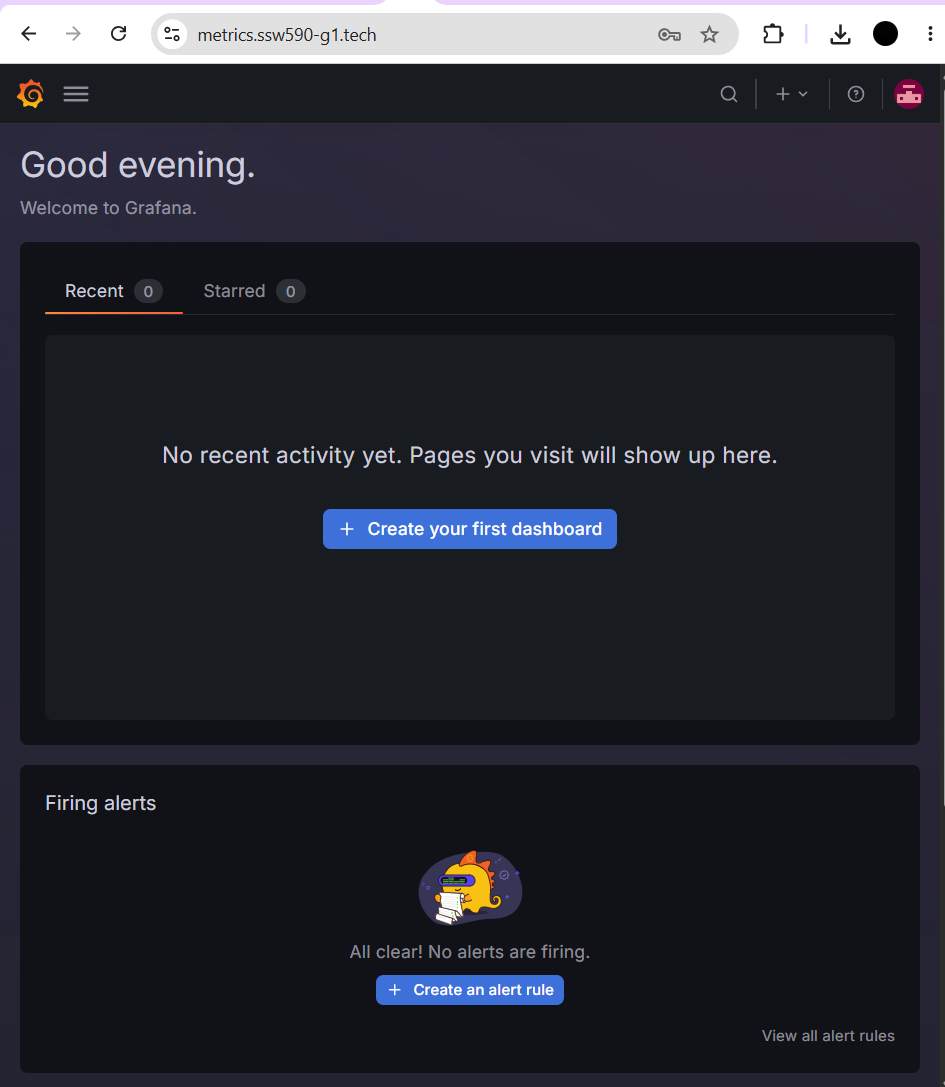
\includegraphics[width=0.85\linewidth]{evidence/144-grafana-admin-signed-in-home-page-no-alerts-firing-bd-2026-11-11.png}
\caption{Grafana home page after BD signed in as administrator over HTTPS with her own password, November 11, 2026 (BD's screenshot).}
\label{Fig:E144}
\end{figure}

% ===== BD region: row 4 =====
% Region: sreDashboard (single owner; edit only your own region)
\section{Dashboard (15 points)}\label{Section:sreDashboard}
\textbf{Owner:} BD. \textbf{Status:} dashboard built and checked November 11, 2026; normal-build comparison \StatusPending.

\paragraph{Dashboard and data source.} The dashboard \emph{Group 1 Startup Server (SRE)} was imported into Grafana from a
JSON file (\texttt{config/monitoring/grafana/group1-sre-dashboard.json}), after the Prometheus data source was added with the
private address \texttt{http://prometheus:9090} (inside the Grafana container, \texttt{localhost} is Grafana itself, not Prometheus).
The time zone is fixed to \texttt{America/New\_York} (shown as EST), the default range is the last 3 hours, and the page refreshes every 30~s
(the scrape interval). Thresholds are drawn as lines on the panels and legends are on. The dashboard definition is kept as JSON in Gitea
(folder \href{\GiteaURL/group1-startup/infra/src/branch/main/monitoring/grafana}{\texttt{monitoring/grafana}} of the \texttt{infra} repository, together with the alert-rules export; added by
\href{\GiteaURL/group1-startup/infra/pulls/5}{pull request \#5}, approved by SD, who found the files identical to the live dashboard and rules and free of secrets, and merged by BD on November 11, 2026, 21:02~EST, as merge commit
\href{\GiteaURL/group1-startup/infra/commit/ff85de447d738e20c2a5cd42b0c8a6d58afd6b3c}{\texttt{ff85de4}}), because screenshots alone cannot restore a dashboard.
\FigRef{145} and \FigRef{146} show the result; the first copy was deleted and imported again after the scrape-health table was widened.

\begin{figure}[htbp]
\centering
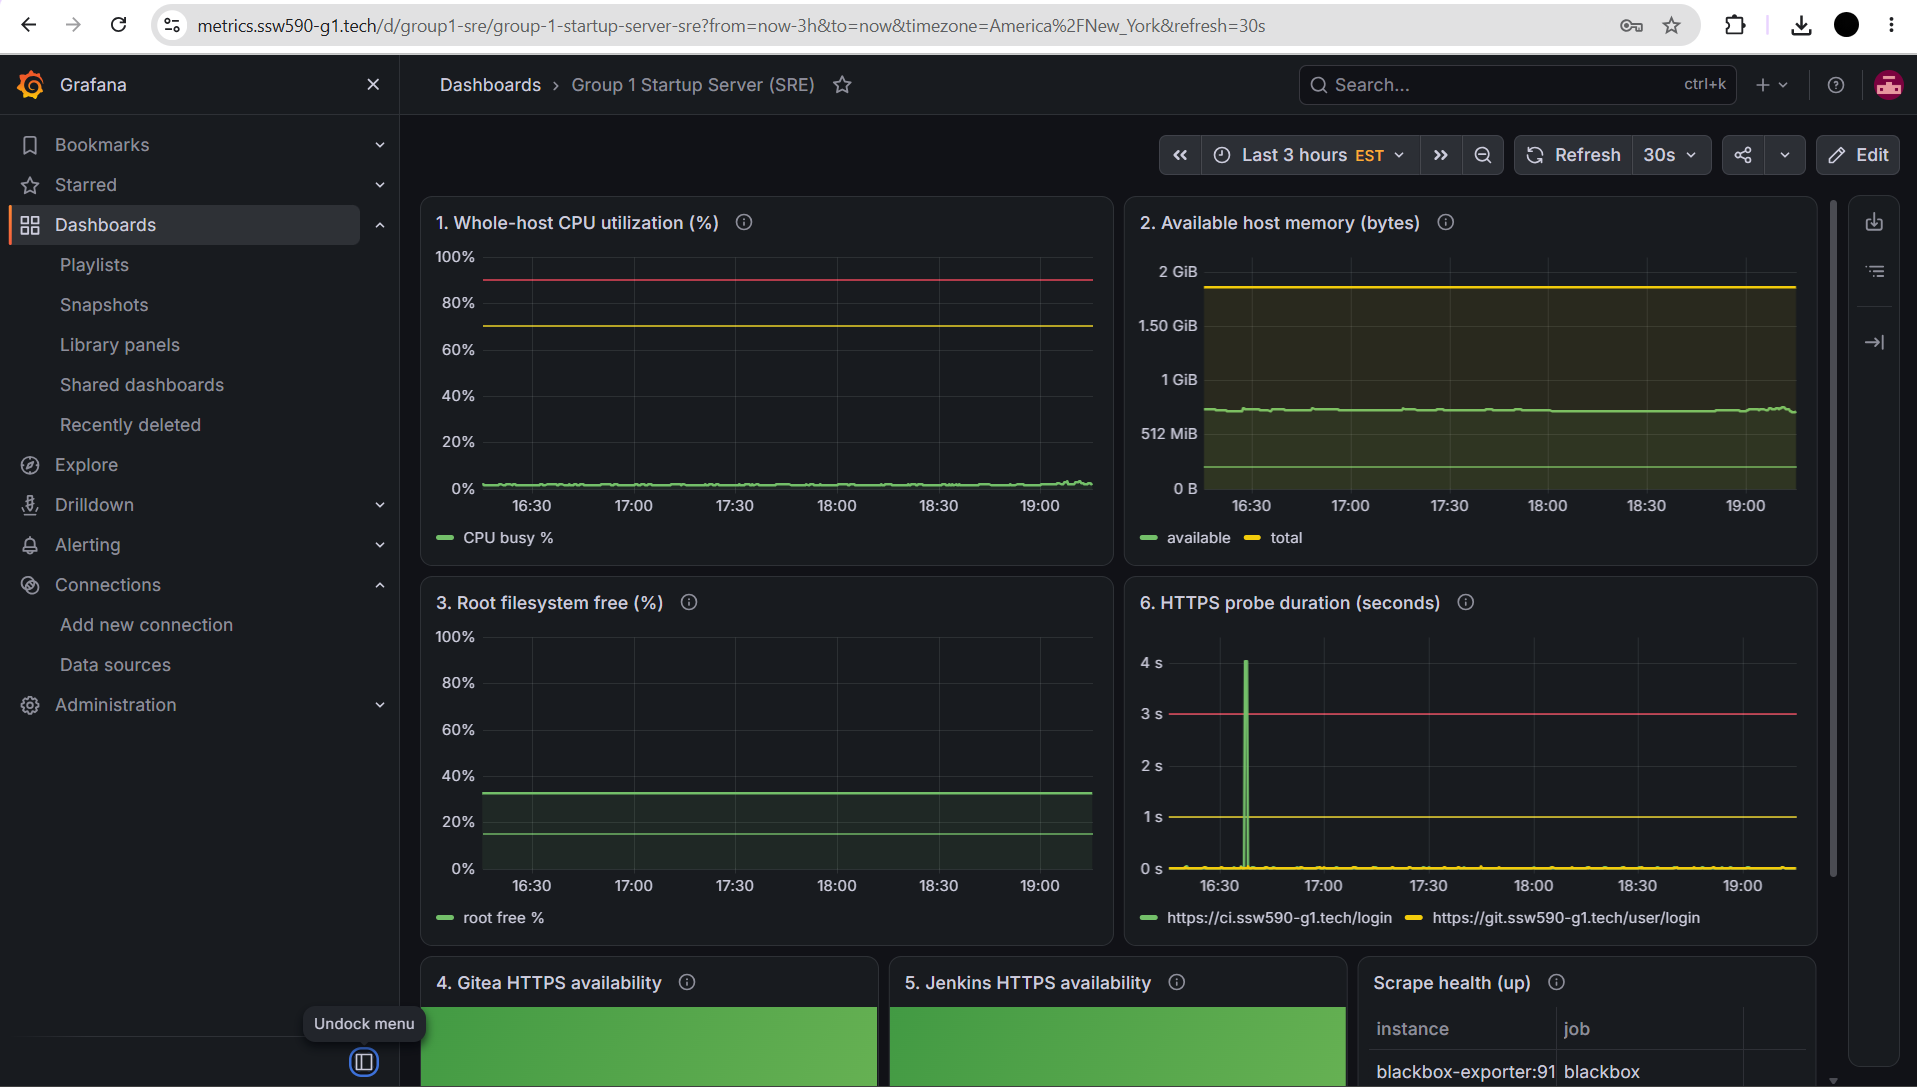
\includegraphics[width=\linewidth]{evidence/145-grafana-dashboard-group1-sre-panels-1-2-3-6-top-half-bd-2026-11-11.png}
\caption{Dashboard, top half, November 11, 2026, last 3 hours EST: CPU about 2\%, available memory about 750~MiB of 1.86~GiB, root filesystem free about 33\%, probe duration of both URLs (one 4~s sample on the Jenkins line).}
\label{Fig:E145}
\end{figure}

\begin{figure}[htbp]
\centering
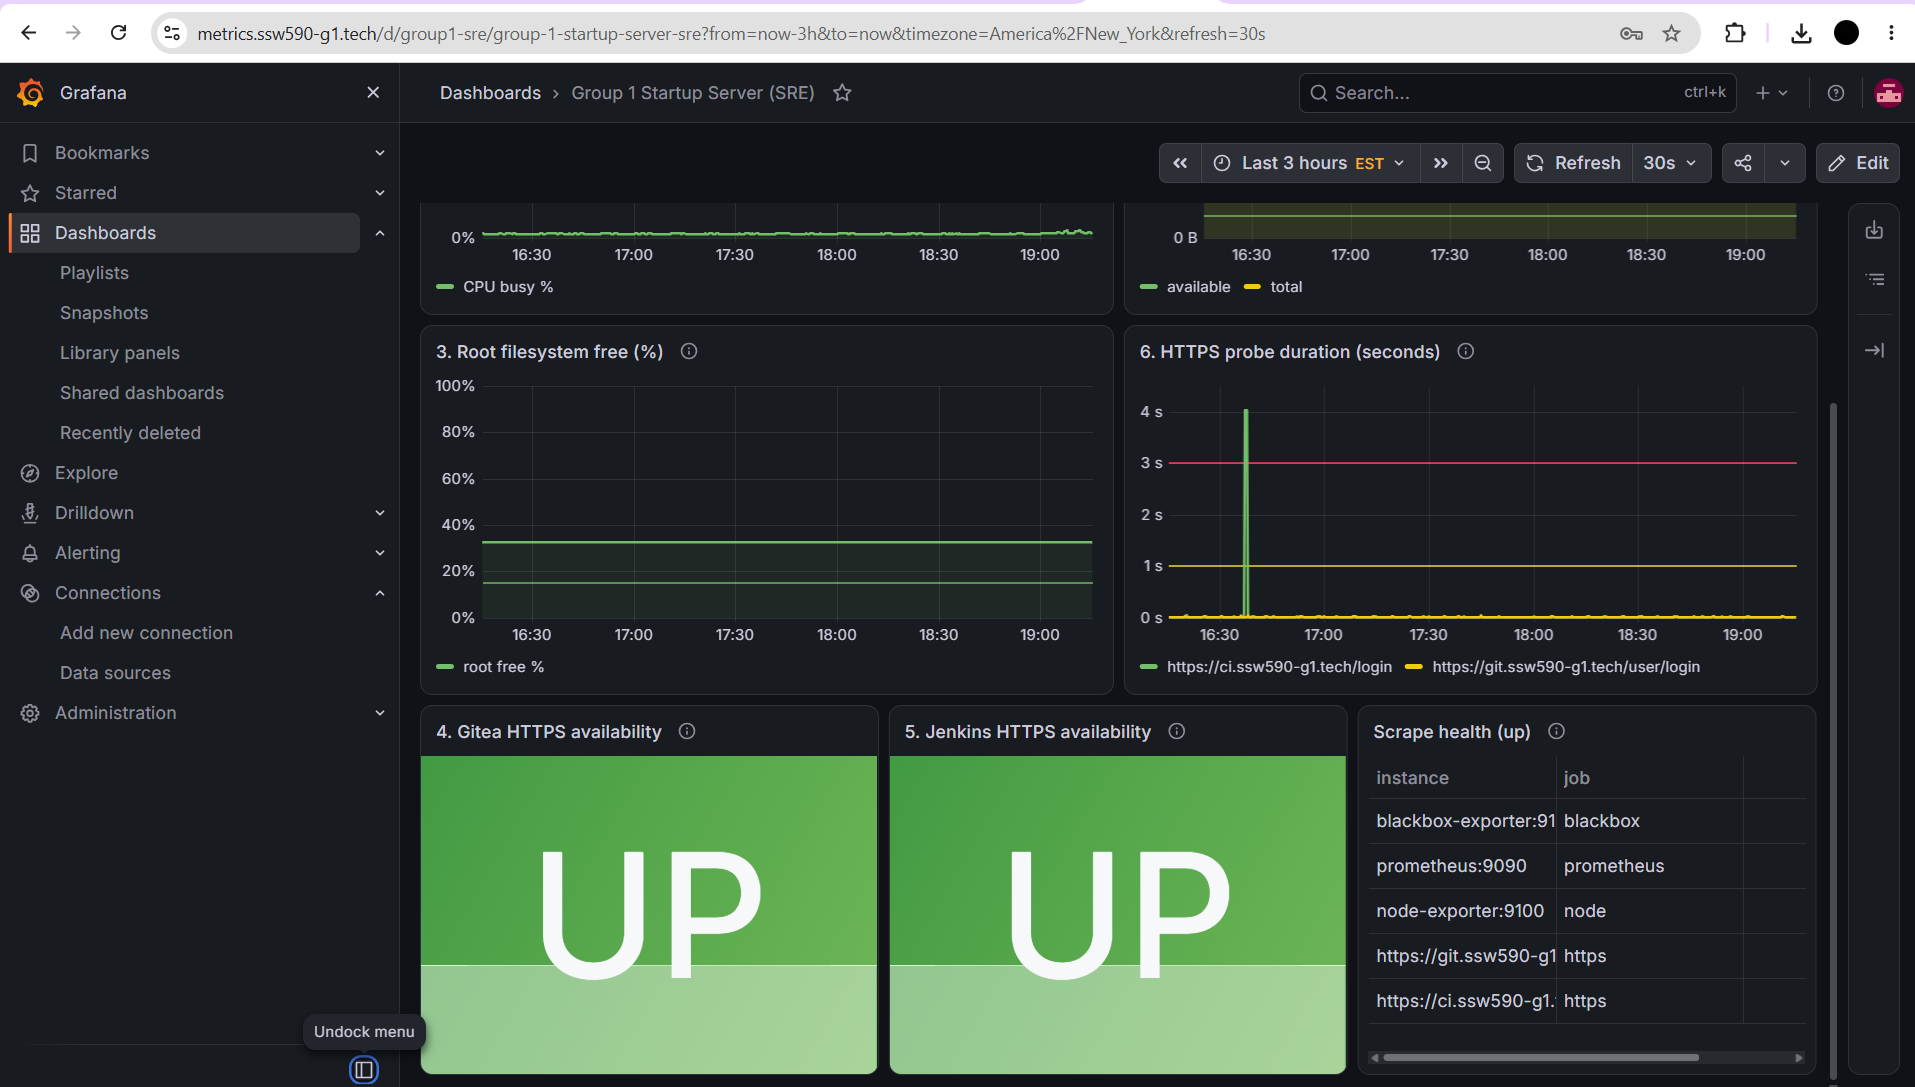
\includegraphics[width=\linewidth]{evidence/146-grafana-dashboard-group1-sre-panels-3-4-5-6-scrape-health-bd-2026-11-11.png}
\caption{Dashboard scrolled down: Gitea and Jenkins both UP, probe duration with two labeled lines, and the scrape-health table.}
\label{Fig:E146}
\end{figure}

\paragraph{The six required panels and their queries.} Each query was run against Prometheus' own API before it went into the
dashboard and compared with \texttt{free -b} and \texttt{df -B1 /} (\ListRef{142}).

\begin{tabularx}{\linewidth}{L{0.6cm}L{3.6cm}Y}
\caption{Dashboard panels and why their queries are written this way\label{Table:SrePanels}}\\
\toprule \textbf{\#} & \textbf{Panel (unit)} & \textbf{Explanation of the query (the queries are in \ListRef{SreQueries})}\\ \midrule
\endfirsthead
\toprule \textbf{\#} & \textbf{Panel (unit)} & \textbf{Explanation}\\ \midrule
\endhead \bottomrule \endlastfoot
1 & Whole-host CPU utilization (percent) & The CPU time counter grows forever, so its rate over 2 minutes is the idle share per second; the average over both CPUs is the host-wide idle share, and 100 times one minus it is the busy percentage. Whole host, not per container.\\
2 & Available host memory (bytes, IEC) & The kernel's estimate of memory applications can still get; it is not the \emph{free} figure. Same value as the \emph{available} column of \texttt{free -b}. Total memory is a second line.\\
3 & Root filesystem free (percent) & Available bytes divided by the size of the same series, the real root filesystem \texttt{/dev/nvme0n1p1} (xfs). The other filesystems (\texttt{/boot/efi}, \texttt{/run}, \texttt{/tmp}) are not mixed in.\\
4 & Gitea HTTPS availability (0 or 1) & 1 means DNS, TLS verification, allowed redirects and the final status all passed. A login-page probe does not prove a Git push.\\
5 & Jenkins HTTPS availability (0 or 1) & The same for the Jenkins login URL; \texttt{/login} is the page Jenkins shows to everyone.\\
6 & HTTPS probe duration (seconds) & One labeled line per URL; a slow response shows before a failure.\\
\end{tabularx}

\begin{longlisting}
\begin{minted}[fontsize=\scriptsize]{text}
1 CPU %      100 * (1 - avg(rate(node_cpu_seconds_total{mode="idle"}[2m])))
2 memory     node_memory_MemAvailable_bytes            (and node_memory_MemTotal_bytes)
3 root free  100 * node_filesystem_avail_bytes{mountpoint="/",fstype!~"tmpfs|overlay|squashfs"}
                 / node_filesystem_size_bytes{mountpoint="/",fstype!~"tmpfs|overlay|squashfs"}
4 Gitea      probe_success{job="https",instance="https://git.ssw590-g1.tech/user/login"}
5 Jenkins    probe_success{job="https",instance="https://ci.ssw590-g1.tech/login"}
6 duration   probe_duration_seconds{job="https"}        (legend: {{instance}})
table        up
\end{minted}
\caption{The dashboard queries (Prometheus query language), as saved in the dashboard JSON.}
\label{Listing:ESreQueries}
\end{longlisting}

The scrape-health table uses \texttt{up}: \texttt{up} is 1 when Prometheus could scrape the target, while \texttt{probe\_success} can be 0 although \texttt{up}
is 1 (the collection worked, the probed request failed). \ListRef{142} lists every filesystem Node Exporter reports and why only the xfs root is used.
Values at 03:29~UTC: CPU 1.69\%, available memory 805,617,664 bytes (\texttt{free}: 806,154,240), root free 32.94\% (7,047,094,272 of 21,395,124,224 bytes),
both probes 1 with 0.012~s and 0.040~s.

\begin{longlisting}
\inputminted[fontsize=\scriptsize]{text}{evidence/142-dashboard-queries-checked-against-prometheus-and-host-bd-2026-11-10.txt}
\caption{Each dashboard query run against Prometheus and compared with \texttt{free -b} and \texttt{df -B1 /}, November 10, 2026 (real output).}
\label{Listing:E142}
\end{longlisting}

\paragraph{Normal Jenkins build.} One normal run of the existing pipeline was captured on a calm server: build \#3 of
\texttt{twintrack/main}, started by BD with \emph{Build Now} on November 12, 2026 at 01:41:47~UTC (November 11, 20:41:47~EST), commit
\texttt{a0094a8} (the merged pull request \#10), result SUCCESS, duration 2.4~s, end about 01:41:49. The console says
\texttt{Running on Jenkins in /var/jenkins\_home/workspace/twintrack\_main}: the build ran on the \emph{controller}, so its resource
use is inside this host's measurements (\FigRef{169}). Jenkins had been up for 14 minutes since its restart in the outage test.
The host values come from Node Exporter's raw samples, one every 30~s (\ListRef{168}):

\begin{tabularx}{\linewidth}{L{3.2cm}L{3.4cm}L{2.6cm}Y}
\caption{Host CPU and available memory around build \#3 (UTC, 30~s samples)\label{Table:SreBuildSamples}}\\
\toprule \textbf{Sample} & \textbf{CPU busy, previous 30~s} & \textbf{Available} & \textbf{Position}\\ \midrule
\endfirsthead
\toprule \textbf{Sample} & \textbf{CPU busy, previous 30~s} & \textbf{Available} & \textbf{Position}\\ \midrule
\endhead \bottomrule \endlastfoot
01:40:46 & 5.7\% & 675~MiB & before\\
01:41:16 & 6.7\% & 671~MiB & before\\
01:41:46 & 5.4\% & 662~MiB & before (1~s before the start)\\
01:42:16 & 10.1\% & 654~MiB & during: the only sample containing the build\\
01:42:46 & 6.2\% & 662~MiB & after\\
01:43:16 & 4.5\% & 695~MiB & after\\
\end{tabularx}

\emph{What changed:} the one sample that contains the 2.4~s build reads 10.1\% CPU, against 4 to 7\% before and after. A one-core job of 2.4~s adds about
$2.4/(30\times 2)=4$ percentage points to a 30~s average over two CPUs, so the rise is of the size expected, but it is a single sample whose neighbours already
vary between 3 and 7\%, so it is consistent with the build and does not prove it. \emph{What did not change:} available memory moved by 10 to 40~MiB, within
the normal movement of the minutes before (632 to 678~MiB). \emph{Why so little is visible:} a build of 2.4~s falls inside one 30~s scrape and is averaged with
27 quiet seconds; the pipeline is two short Python commands. No extra load was created to force a spike. Whole-host figures do not say how much of the CPU belongs to
Jenkins rather than to another container. Other activity in the window (the manual build on the Gitea Actions runner at 01:35 to 01:36 with CPU above 50\%, and a missing
sample at 01:38:46) is listed in \ListRef{168}.
The earlier build \texttt{main} \#2 (01:29:12~UTC, 7.9~s, \FigRef{166}) was \emph{not} used: it ran two minutes after Jenkins was restarted in the outage test, when the host was
already busy with Jenkins' own start-up (CPU 6 to 39\% in the surrounding scrapes), so the build could not be told apart from the restart.

\begin{longlisting}
\inputminted[fontsize=\scriptsize]{text}{evidence/168-normal-jenkins-build-3-host-metrics-before-during-after-bd-2026-11-11.txt}
\caption{Build \#3 of \texttt{main}: facts, host samples before, during and after, interpretation, and the other activity in the window (real output).}
\label{Listing:E168}
\end{longlisting}

\begin{figure}[htbp]
\centering
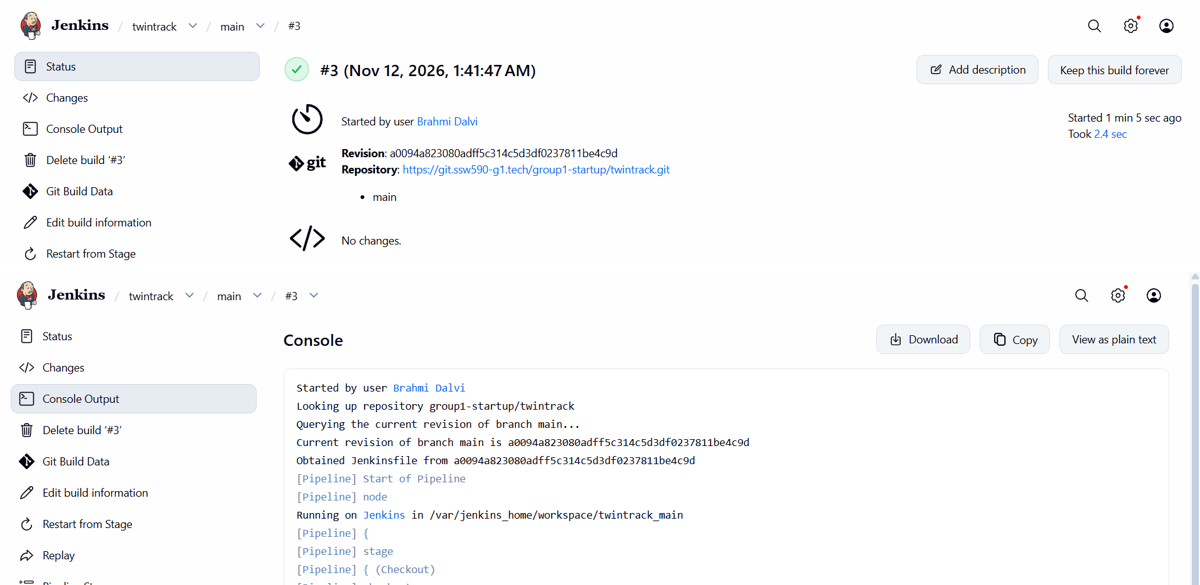
\includegraphics[width=0.9\linewidth]{evidence/169-jenkins-twintrack-main-build-3-success-2-4-s-and-console-running-on-controller-bd-2026-11-12.png}
\caption{Jenkins build \#3 of \texttt{twintrack/main} (Nov 12, 2026, 1:41:47 AM server time): SUCCESS, took 2.4~s, and its console, \texttt{Running on Jenkins in /var/jenkins\_home/workspace/twintrack\_main}, the controller.}
\label{Fig:E169}
\end{figure}

\paragraph{Observation.} The Jenkins probe duration shows one sample of about 4~s (above the 3~s red line) at about 16:25~EST on November 11. Its cause was not investigated; it is reported here instead of being hidden.

% ===== SD region: row 5 =====
% Region: sreSlo (single owner; edit only your own region)
\section{SLI, SLO, and error budget (10 points)}\label{Section:sreSlo}
\index{SLI}\index{SLO}\index{SLA}\index{error budget}
\textbf{Owner:} SD. \textbf{Status:} worked example and a real 18-minute window around the controlled outage \StatusPass.

\paragraph{Definitions.}
\begin{tabularx}{\linewidth}{L{1.4cm}Y}
\toprule \textbf{Term} & \textbf{Meaning here}\\ \midrule
SLI & \emph{Service-level indicator}: a measured fraction. Ours is the share of scheduled HTTPS probes that succeed for one service over a stated window: successful \texttt{probe\_success} samples divided by all samples received.\\
SLO & \emph{Service-level objective}: our internal target for that SLI, at least 99\,\% probe success over a 24-hour window, evaluated separately for Gitea and Jenkins. It is a lab target chosen by the course, not a promise.\\
SLA & \emph{Service-level agreement}: a commitment to a customer, usually with consequences if missed. This startup has no customer SLA; nothing here is one.\\ \bottomrule
\end{tabularx}
\paragraph{How the SLI is computed.} For one service and a window \texttt{W}, with one sample every 30~seconds:
\begin{minted}{text}
100 * avg_over_time(probe_success{job="https", instance="https://ci.ssw590-g1.tech/login"}[W])
count_over_time(probe_success{job="https", instance="https://ci.ssw590-g1.tech/login"}[W])   # samples received
\end{minted}
\texttt{probe\_success} is 1 or 0, so its average over the window is the success fraction. The count is compared with the
expected number of samples (\texttt{W} / 30\,s); a missing sample is unknown, not a success. Dashboard panels~4 and~5
(Section~\ref{Section:sreDashboard}) show the same series sample by sample.

\paragraph{What this SLI does not see.} It measures availability of the login page, not speed. A probe that takes
4~seconds but returns 200 still counts as a success: the Jenkins probe did exactly that once on Nov~11 near 16:25~EST
(dashboard panel~6), and the availability SLI did not change. Catching slowness would need a second, latency SLI, for
example the share of probes faster than 1~second. A login page that loads also does not prove that a Git push or a build works.

The difference in one line: the SLI is what we measure, the SLO is the target we hold ourselves to, and an SLA is what we would owe
someone else if we missed it \cite{GoogleSREWorkbookSLO}.

\paragraph{Worked example (hypothetical numbers from the course manual, not our results).}
A probe every 30~seconds for 24~hours gives $24 \times 60 \times 2 = 2{,}880$ scheduled probes per service.
\begin{itemize}[nosep]
  \item \textbf{Gitea:} 2,880 successes out of 2,880 probes, so the SLI is $100 \times 2880/2880 = 100\,\%$. It meets the 99\,\% SLO.
  \item \textbf{Jenkins:} 2,850 successes and 30 failures, so the SLI is $100 \times 2850/2880 \approx 98.96\,\%$. It misses the SLO, by about 0.04 percentage points.
  \item \textbf{Error budget:} a 99\,\% SLO allows 1\,\% of probes to fail: $0.01 \times 2880 = 28.8$ failed samples. Because each sample stands for 30~seconds, that is $28.8 \times 0.5 = 14.4$ minutes of failure in the day, if failures are spread evenly across samples.
  \item \textbf{Jenkins over budget:} 30 failures use $30 - 28.8 = 1.2$ samples (about 0.6 minutes) more than the budget. Samples are whole, so at most 28 failed samples ($100 \times 2852/2880 \approx 99.03\,\%$) would still meet the target; 29 would not ($\approx 98.99\,\%$).
\end{itemize}
The budget is a way to decide, not just a score: while Jenkins has budget left, the team can accept risky changes; once it is
spent, reliability work comes first.

\paragraph{Our short window.} The real window was agreed with BD around her controlled Jenkins outage
(Section~\ref{Section:sreIncident}): November 11, 2026, 8:20:00 to 8:38:00~PM New York time (01:20:00 to 01:38:00~UTC on
November 12), 18~minutes. Jenkins was stopped at 8:24:25 and started again at 8:27:25~PM. The queries above were evaluated
at the end of the window, with \texttt{W = 1080s}, once the window had closed and before the restart test of
Section~\ref{Section:sreDeployment} could add a gap (\ListRef{116}).

\begin{tabularx}{\linewidth}{L{2.0cm}L{2.0cm}L{1.6cm}L{1.6cm}L{1.6cm}Y}
\caption{SLI for the window 8:20--8:38~PM, November 11, 2026\label{Table:SreWindow}}\\
\toprule \textbf{Service} & \textbf{Samples (expected)} & \textbf{Success} & \textbf{Failed} & \textbf{SLI} & \textbf{99\,\% budget for 36 samples}\\ \midrule
\endfirsthead
\toprule \textbf{Service} & \textbf{Samples (expected)} & \textbf{Success} & \textbf{Failed} & \textbf{SLI} & \textbf{99\,\% budget for 36 samples}\\ \midrule
\endhead \bottomrule \endlastfoot
Gitea & 36 (36) & 36 & 0 & 100.00\,\% & 0.36 allowed, 0 used: within\\
Jenkins & 36 (36) & 30 & 6 & 83.33\,\% & 0.36 allowed, 6 used: over\\
\end{tabularx}

No sample was missing, so no part of the window is unknown. The 6 failed Jenkins samples are $6 \times 30 = 180$~seconds,
matching the 3-minute outage; the probe got HTTP 502 from Caddy, so the failure was Jenkins itself, not DNS, TLS, or the
proxy (\ListRef{117}). Gitea was not affected. A window this short cannot establish the 24-hour SLO: one failed sample
already exceeds its 0.36-sample budget. Measured over a full day of 2,880 probes, the same 6 failures would give
$100 \times 2874/2880 \approx 99.79\,\%$, inside the 28.8-sample budget of the worked example.

\begin{longlisting}
\inputminted[fontsize=\scriptsize]{text}{evidence/116-sli-window-around-controlled-jenkins-outage-sd-2026-11-11.txt}
\caption{SLI for the window around the controlled Jenkins outage: PromQL, evaluation time, coverage, successes, failures, November 11, 2026 (real output).}
\label{Listing:E116}
\end{longlisting}

\begin{longlisting}
\inputminted[fontsize=\scriptsize]{text}{evidence/117-outage-timeline-recorder-probe-and-container-state-sd-2026-11-11.txt}
\caption{Independent outage timeline from a read-only recorder: Jenkins container state, probe values, and direct HTTPS checks every 15 seconds, November 11, 2026 (real output).}
\label{Listing:E117}
\end{longlisting}

% ===== BD region: rows 6, 7 =====
% Region: sreAlerts (single owner; edit only your own region)
\section{Alerts (15 points)}\label{Section:sreAlerts}
\textbf{Owner:} BD. \textbf{Status:} both rules fired, delivered and resolved on November 11, 2026 \StatusPass.

\paragraph{Contact point and routing.} One contact point, \texttt{team-alerts}, uses Grafana's dedicated \emph{Discord} integration (no SMTP is needed)
and posts to the private Discord channel of the team (BD owns the server; SD was sent an invitation on November 11, 2026); resolved notifications stay on. The channel's webhook URL is a secret: it was
pasted only into Grafana, is stored in Grafana's volume, and is in no repository, screenshot or this PDF (\FigRef{149}; Grafana hides it). The default
notification policy sends everything to \texttt{team-alerts} (the built-in contact point \texttt{empty} has no integration and is unused), groups by folder and alert
name, waits 30~s before the first message, 1~minute before updates, and repeats every 4~hours (\FigRef{151}). A test message arrived in Discord (\FigRef{150}),
which proves delivery only; the rule tests below prove the queries, thresholds and routing.

\begin{figure}[htbp]
\centering
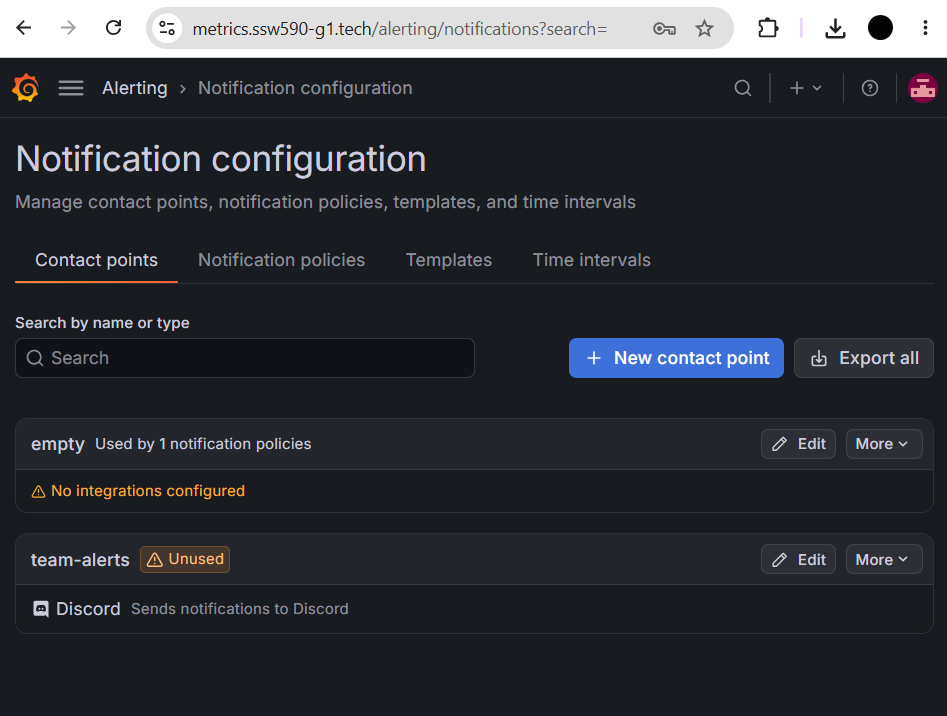
\includegraphics[width=0.8\linewidth]{evidence/149-grafana-contact-point-team-alerts-discord-saved-bd-2026-11-11.png}
\caption{Contact points: \texttt{team-alerts} with one Discord integration (the webhook URL is not shown); \texttt{empty} has no integrations.}
\label{Fig:E149}
\end{figure}

\begin{figure}[htbp]
\centering
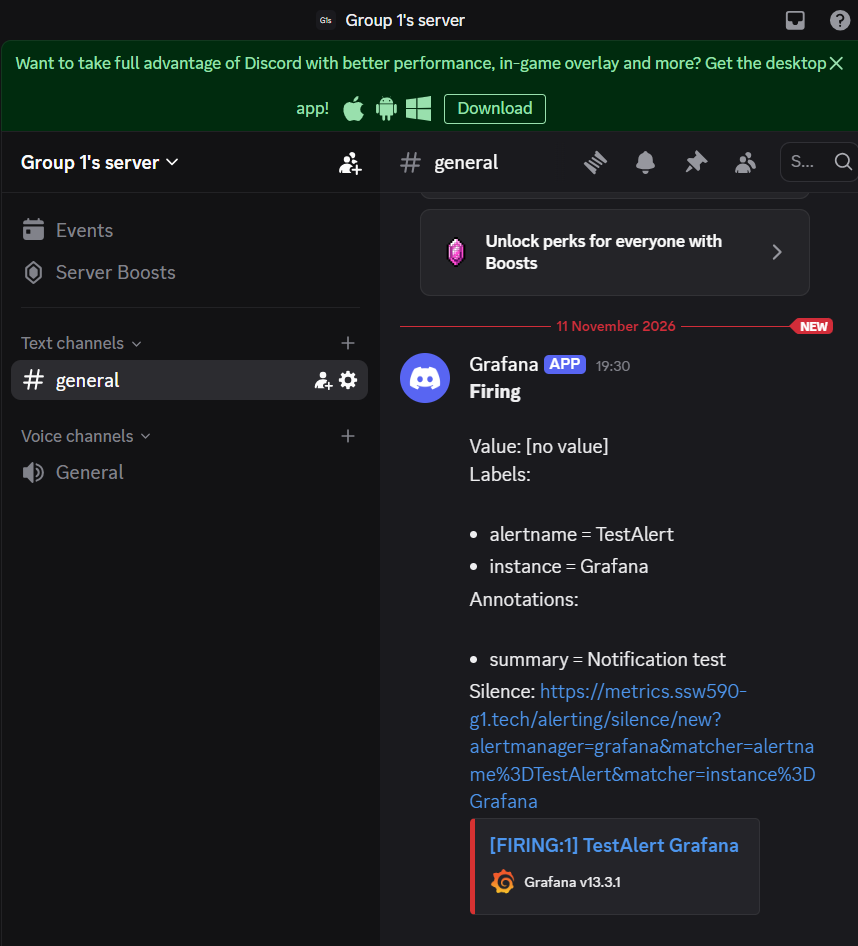
\includegraphics[width=0.8\linewidth]{evidence/150-discord-contact-point-test-notification-received-bd-2026-11-11.png}
\caption{Grafana's test notification in the Discord channel, November 11, 2026, 19:30 EST.}
\label{Fig:E150}
\end{figure}

\begin{figure}[htbp]
\centering
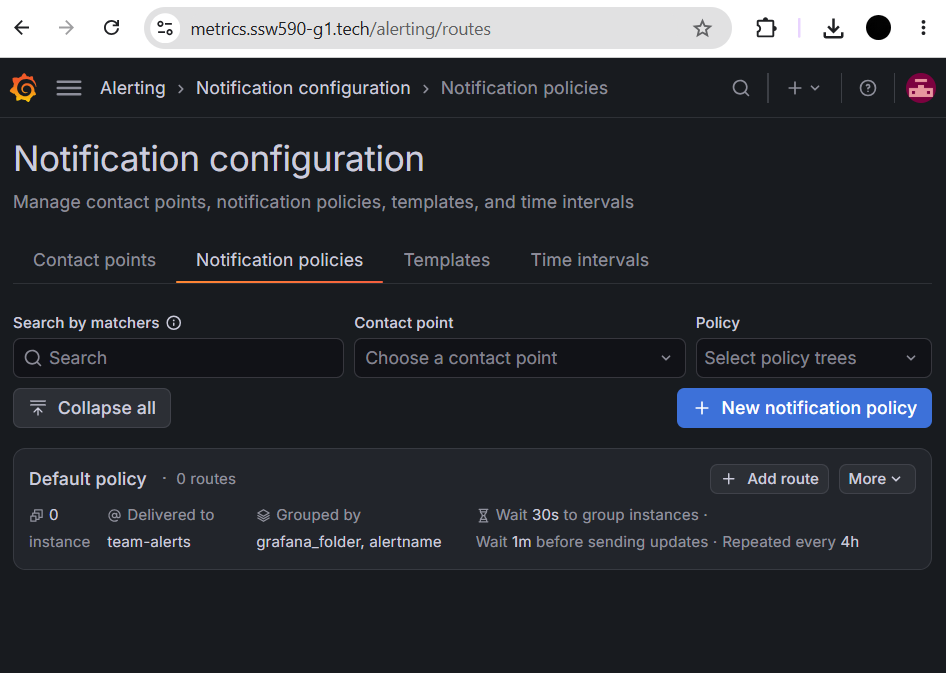
\includegraphics[width=0.8\linewidth]{evidence/151-grafana-default-notification-policy-team-alerts-timing-bd-2026-11-11.png}
\caption{Default notification policy: delivered to \texttt{team-alerts}, grouped by \texttt{grafana\_folder} and \texttt{alertname}, group wait 30~s, group interval 1~m, repeat 4~h.}
\label{Fig:E151}
\end{figure}

\paragraph{The two rules.} Both rules are Grafana-managed, live in the folder \emph{Group 1}, and are exported as YAML
(\texttt{config/monitoring/grafana/alert-rules.yaml}) so that they can be restored.

\begin{tabularx}{\linewidth}{L{2.6cm}YY}
\caption{Alert rules: owner, severity, query, threshold, timing, no-data policy\label{Table:SreRules}}\\
\toprule \textbf{Item} & \textbf{\texttt{https-service-down}} & \textbf{\texttt{root-disk-below-15-percent}}\\ \midrule
\endfirsthead
\toprule \textbf{Item} & \textbf{\texttt{https-service-down}} & \textbf{\texttt{root-disk-below-15-percent}}\\ \midrule
\endhead \bottomrule \endlastfoot
Owner, severity & Brahmi Dalvi; \texttt{critical} & Brahmi Dalvi; \texttt{warning}\\
Query & \texttt{\small probe\_success\{job="https"\}}: one alert per \texttt{instance} (Gitea, Jenkins) & the root-filesystem free-percentage query of panel~3 (\texttt{/dev/nvme0n1p1}, xfs only)\\
Threshold & below 1 & below 15 (percent free)\\
Evaluation, pending & every 30~s; pending 1~minute & every 1~minute; pending 5~minutes\\
No data, error & \texttt{NoData} and \texttt{Error}: each raises its own alert to \texttt{team-alerts}, so a missing series or failed collection is reported and never read as healthy & the same\\
Summary & \texttt{\{\{ \$labels.instance \}\} failed its HTTPS probe for at least 1 minute} & Root filesystem has less than 15\% free\\
Operator response & check the container (\texttt{docker ps}, \texttt{docker logs}), HTTPS from outside, Caddy and the certificate; restart the container; see Section~\ref{Section:sreIncident} & \texttt{docker system df}; remove unused images only after checking they are not the runner's image; check Prometheus (1~GB cap) and logs; never delete volumes\\
Runbook link & the \texttt{runbook\_url} annotation of both rules points to this manual's repository \texttt{\GiteaURL/group1-startup/manual}; the response steps are the row above and Section~\ref{Section:sreIncident} & the same\\
\end{tabularx}

\FigRef{152} to \FigRef{155} show both saved rules (state, query, threshold, pending period, no-data and error states, annotations).

\begin{figure}[htbp]
\centering
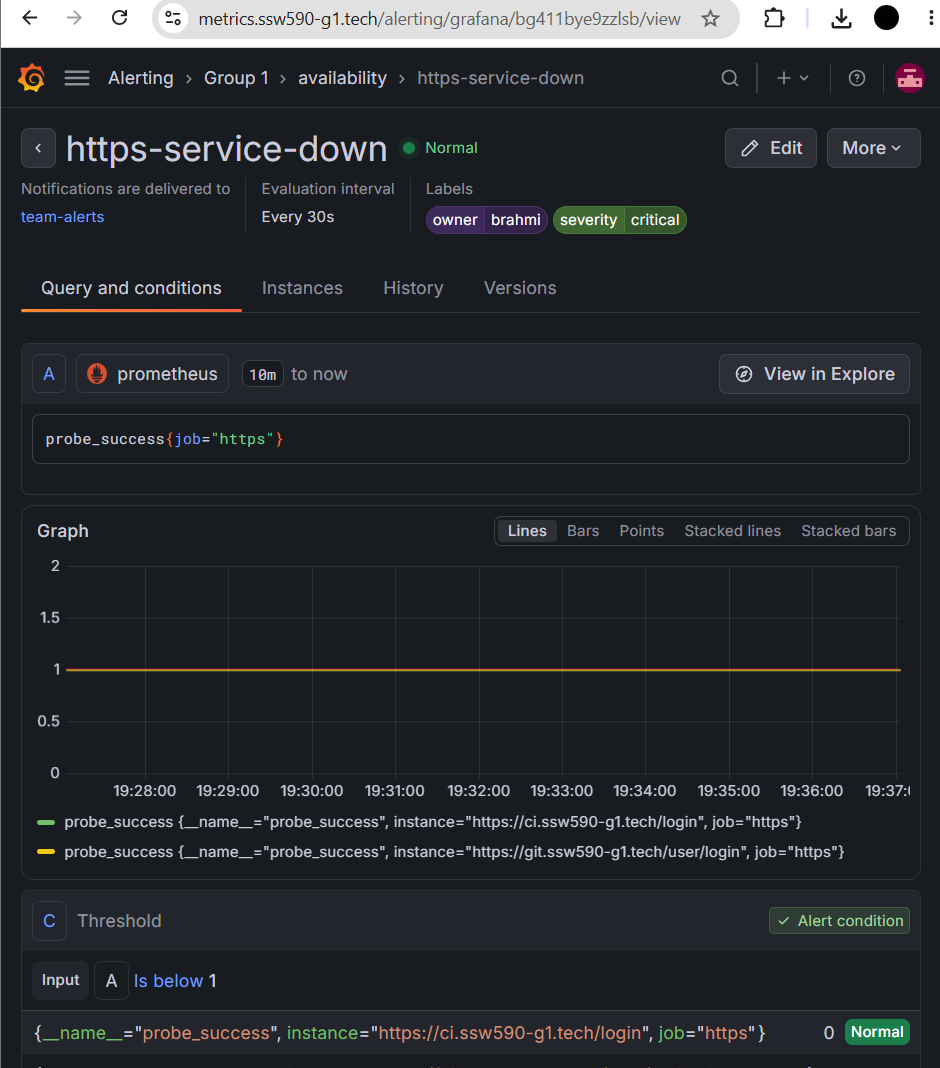
\includegraphics[width=0.85\linewidth]{evidence/152-grafana-alert-rule-https-service-down-query-threshold-labels-bd-2026-11-11.png}
\caption{Rule \texttt{https-service-down}: query, threshold ``below 1'', labels \texttt{owner} and \texttt{severity}, notifications to \texttt{team-alerts}.}
\label{Fig:E152}
\end{figure}

\begin{figure}[htbp]
\centering
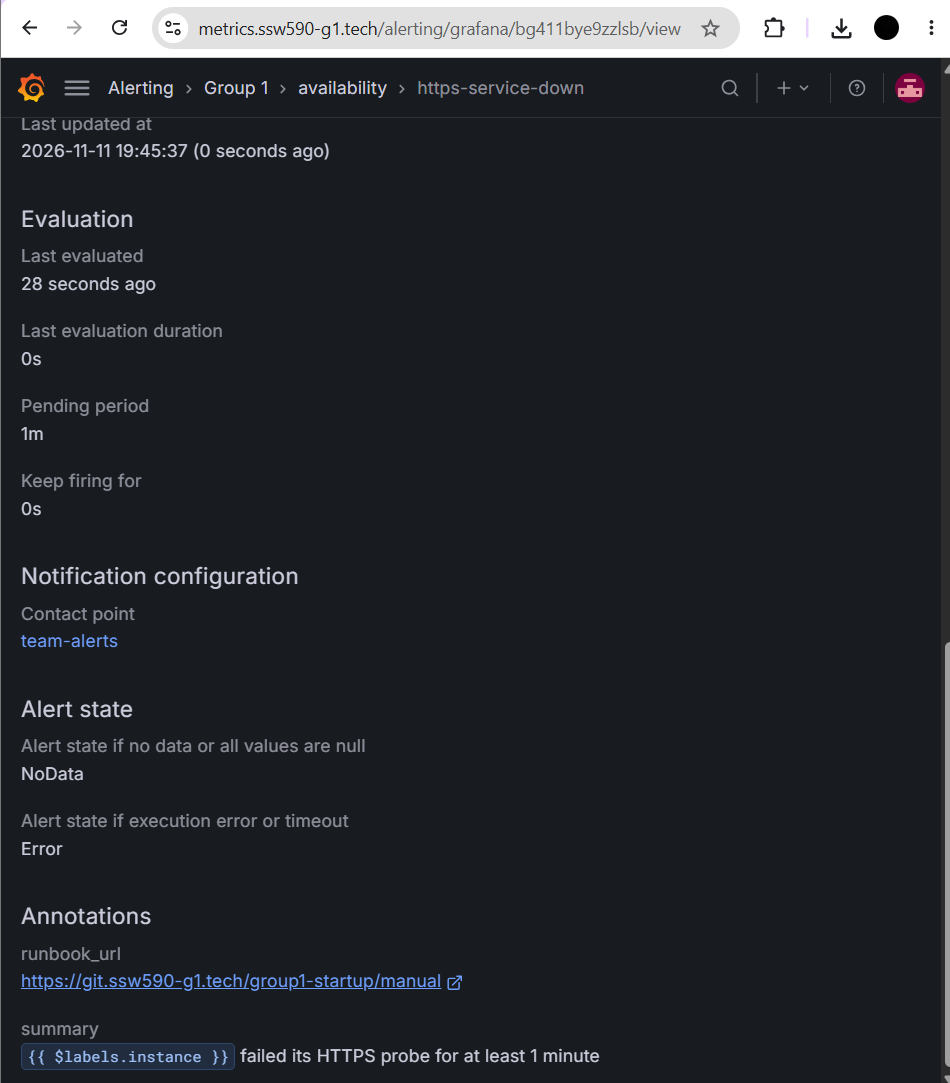
\includegraphics[width=0.85\linewidth]{evidence/153-grafana-alert-rule-https-service-down-pending-nodata-error-summary-runbook-bd-2026-11-11.png}
\caption{The same rule, lower part: pending 1~m, no data \texttt{NoData}, error \texttt{Error}, \texttt{runbook\_url} and \texttt{summary}.}
\label{Fig:E153}
\end{figure}

\begin{figure}[htbp]
\centering
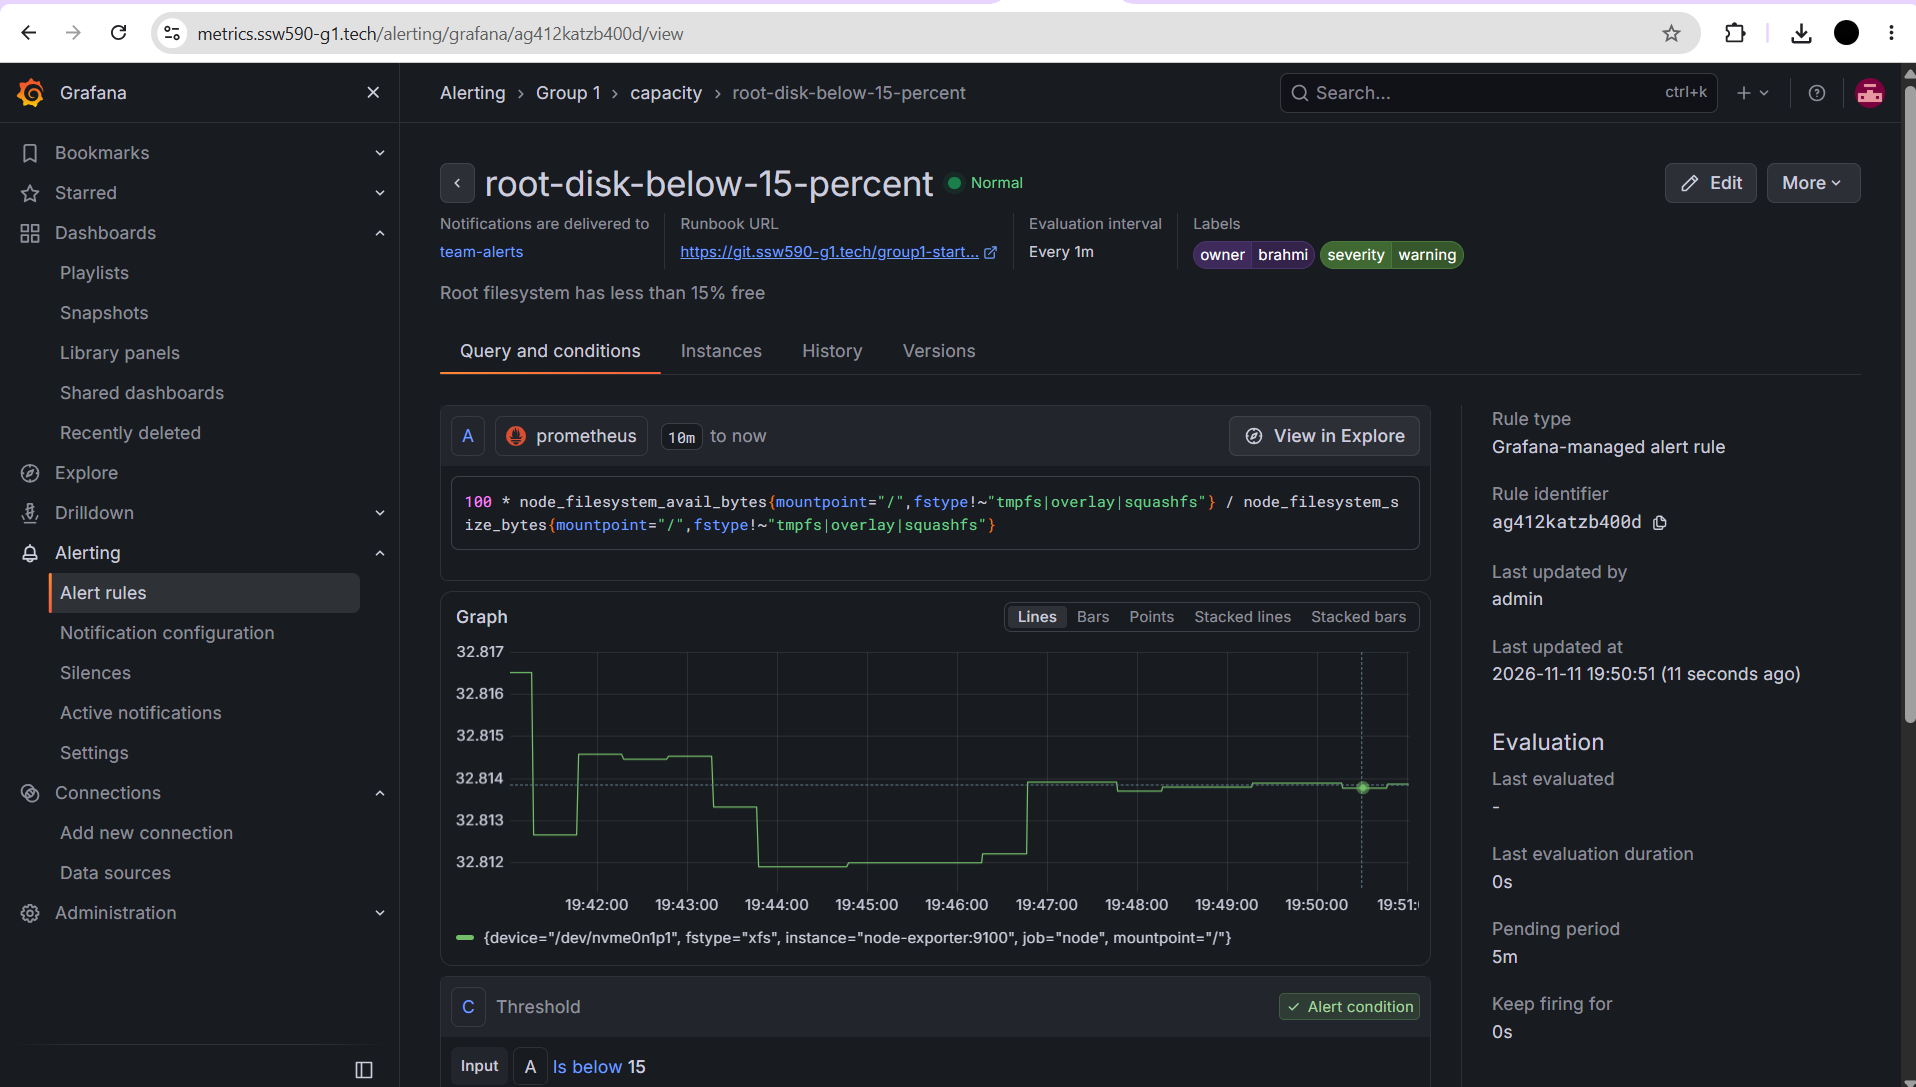
\includegraphics[width=0.85\linewidth]{evidence/154-grafana-alert-rule-root-disk-below-15-percent-query-labels-graph-bd-2026-11-11.png}
\caption{Rule \texttt{root-disk-below-15-percent}: query for the xfs root, graph at about 32.8\%, threshold ``below 15''.}
\label{Fig:E154}
\end{figure}

\begin{figure}[htbp]
\centering
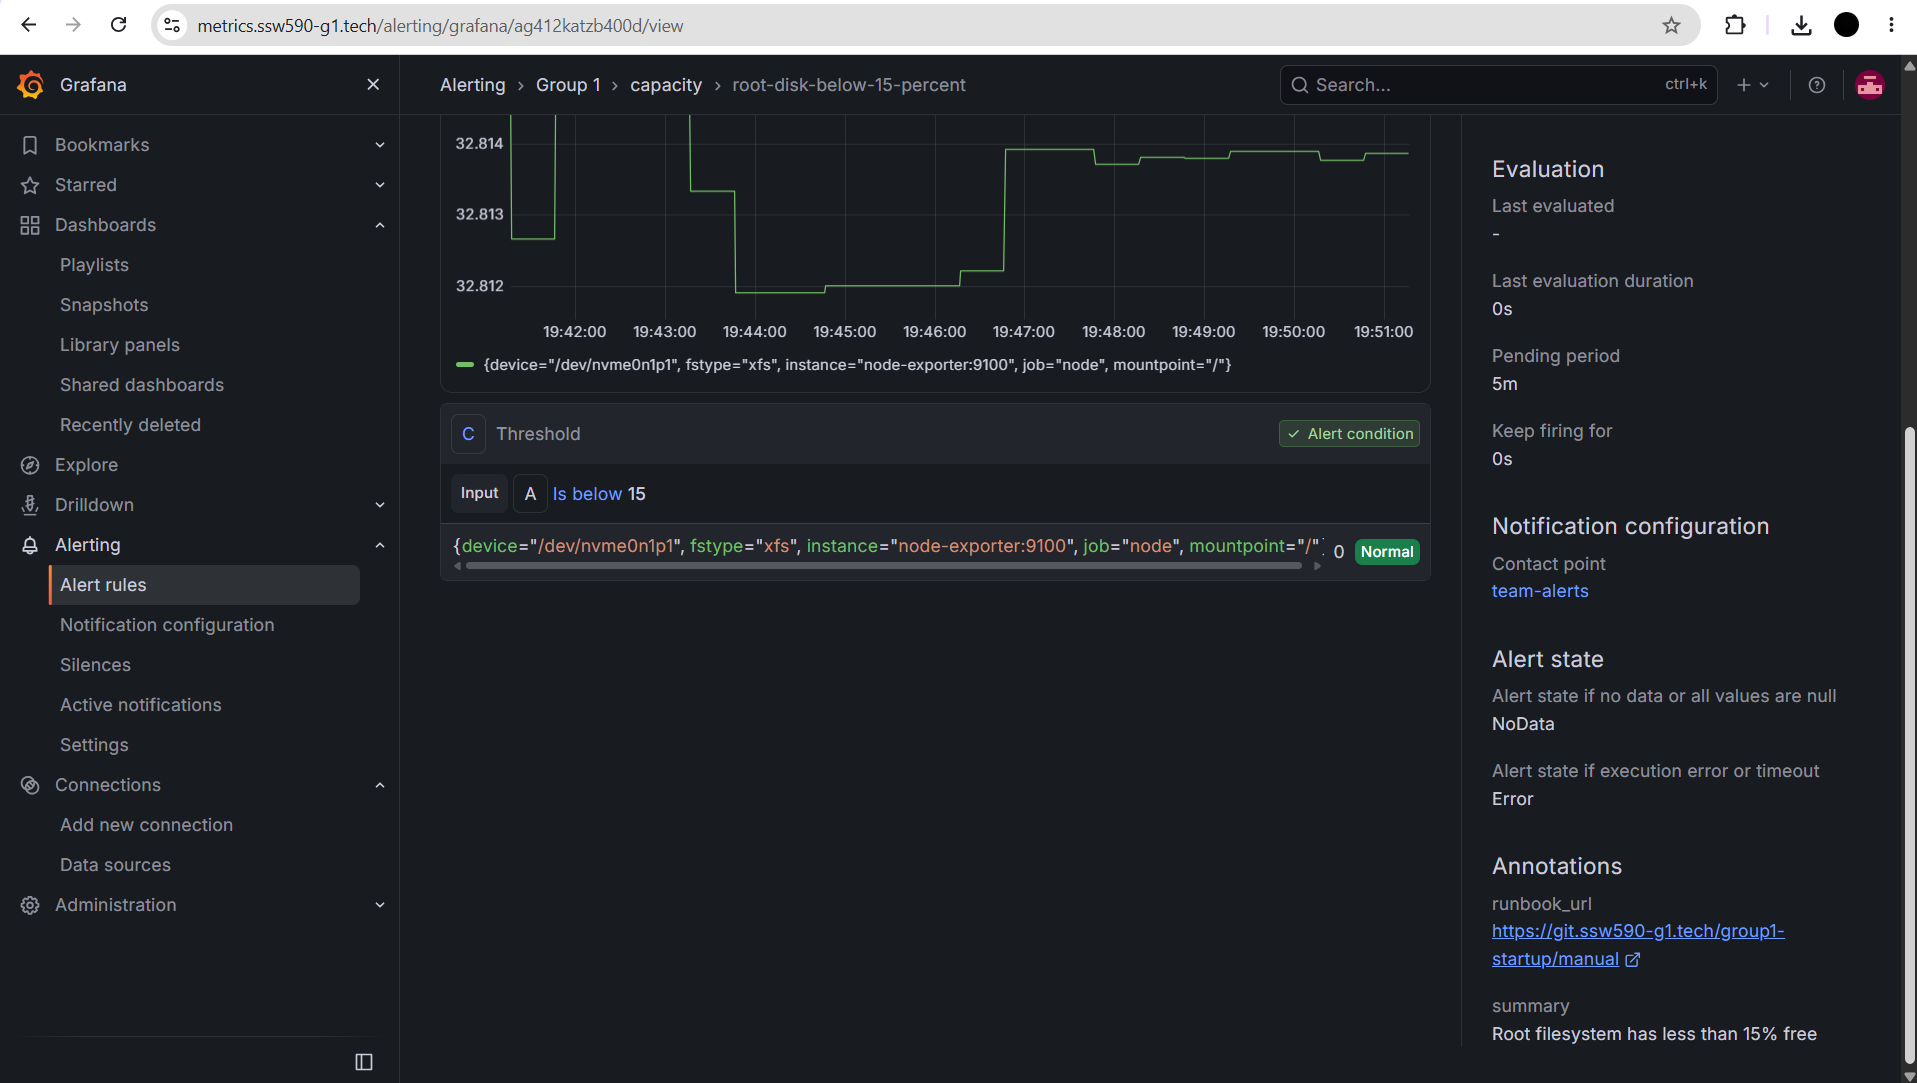
\includegraphics[width=0.85\linewidth]{evidence/155-grafana-alert-rule-root-disk-below-15-percent-pending-nodata-error-annotations-bd-2026-11-11.png}
\caption{The same rule, lower part: pending 5~m, \texttt{NoData}, \texttt{Error}, \texttt{runbook\_url}, \texttt{summary}.}
\label{Fig:E155}
\end{figure}

\paragraph{Test 1: host capacity, with a temporary threshold.} The disk was never filled. On November 11, 2026 the threshold was raised from 15 to 55 percent
(the disk had about 33\% free) at 20:02:10~EST; the rule went to Pending at 20:02:30 and to Alerting after exactly the 5-minute pending period at 20:07:30; the Discord message arrived at 20:08
(\FigRef{157}); the threshold was restored to 15 at 20:15:20, the rule was Normal at once, and the Resolved message arrived at 20:16 (\ListRef{162}). The Resolved message says
\texttt{grafana\_state\_reason = Updated}: the alert cleared because the rule was edited back, which is the planned way to test resolution. The final threshold is 15.

\begin{longlisting}
\inputminted[fontsize=\scriptsize]{text}{evidence/162-disk-alert-test-timeline-threshold-55-then-restored-15-bd-2026-11-11.txt}
\caption{Real timeline of the disk-capacity test: raised to 55, Pending, Firing, Discord, restored to 15, Normal, Resolved.}
\label{Listing:E162}
\end{longlisting}

\begin{figure}[htbp]
\centering
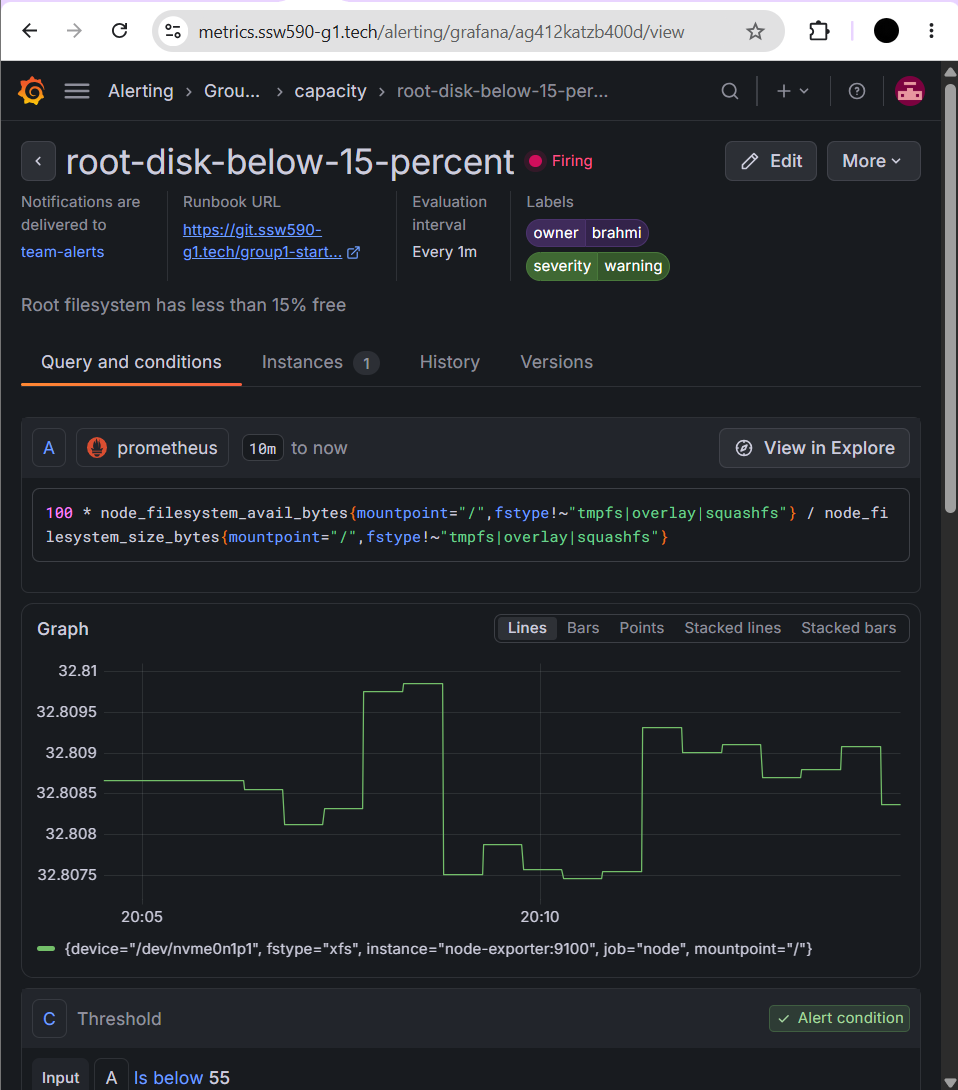
\includegraphics[width=0.8\linewidth]{evidence/157-grafana-disk-rule-firing-threshold-55-bd-2026-11-11.png}
\caption{Disk rule Firing with the temporary threshold 55, 20:08 EST.}
\label{Fig:E157}
\end{figure}

\begin{figure}[htbp]
\centering
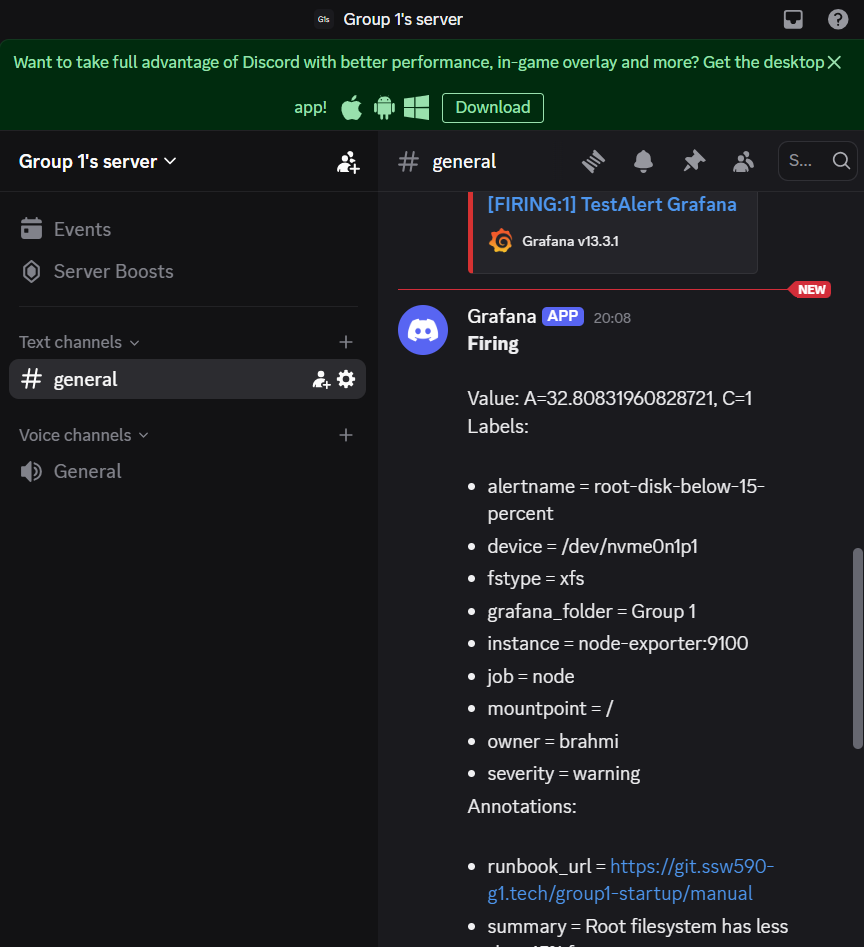
\includegraphics[width=0.8\linewidth]{evidence/158-discord-disk-alert-firing-notification-20-08-bd-2026-11-11.png}
\caption{The Discord Firing message for the disk rule, 20:08 EST.}
\label{Fig:E158}
\end{figure}

\begin{figure}[htbp]
\centering
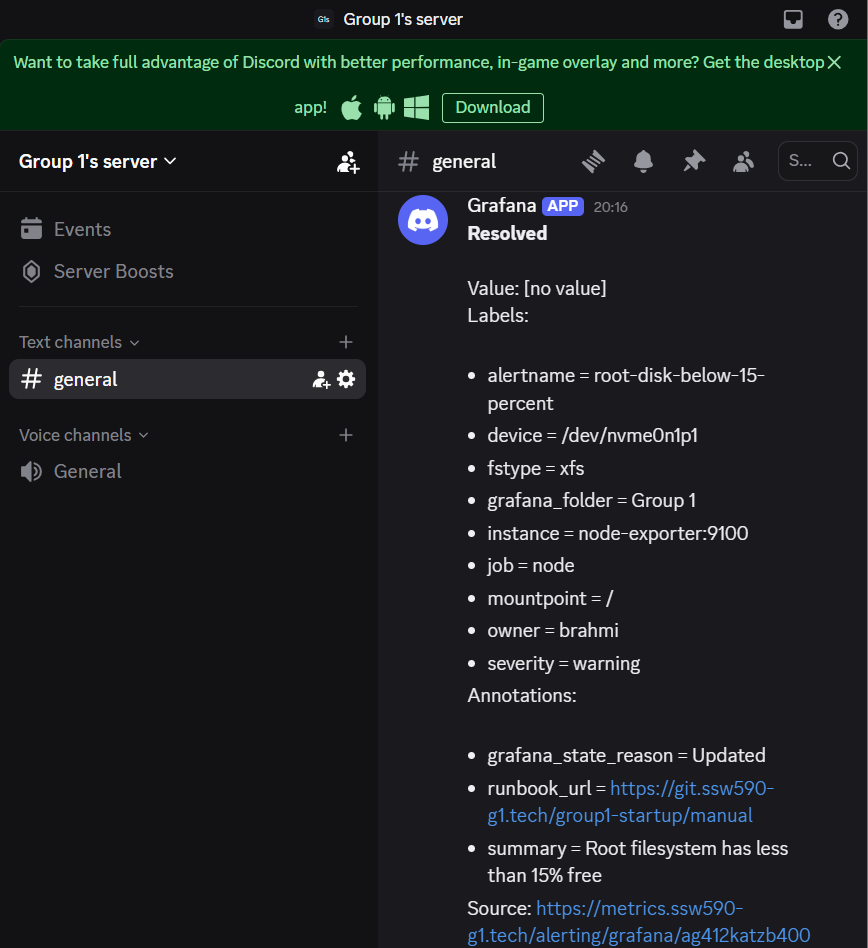
\includegraphics[width=0.8\linewidth]{evidence/160-discord-disk-alert-resolved-notification-20-16-bd-2026-11-11.png}
\caption{The Discord Resolved message, 20:16 EST, after the threshold was restored to 15.}
\label{Fig:E160}
\end{figure}

\paragraph{Test 2: service availability.} The second rule was tested by the controlled Jenkins outage (Section~\ref{Section:sreIncident}): it went Pending at 20:25:10~EST, Firing at 20:26:10, a Discord message
arrived at 20:26 (\FigRef{164}), and after the restart the rule was Normal at 20:28:10 with a Resolved message at 20:28 (\FigRef{165}, \FigRef{163}).

% Region: sreIncident (single owner; edit only your own region)
\section{Controlled incident and review (10 points)}\label{Section:sreIncident}
\textbf{Owner:} BD, with SD recording. \textbf{Status:} outage run and verified November 11, 2026; blameless review and issues \StatusPending.

\paragraph{Exercise.} BD and SD agreed, both being on campus, to stop only the Jenkins container for about three minutes. No build was running. Gitea and monitoring stayed up; no volume was
touched and the instance was not stopped. BD ran \texttt{docker stop jenkins} and, after the Discord message, \texttt{docker start jenkins} in an SSH session, each with the time printed by \texttt{date -u}.

\begin{tabularx}{\linewidth}{L{2.4cm}L{1.9cm}Y}
\caption{Incident timeline, November 11 to 12, 2026\label{Table:SreTimeline}}\\
\toprule \textbf{UTC} & \textbf{EST} & \textbf{Event}\\ \midrule
\endfirsthead
\toprule \textbf{UTC} & \textbf{EST} & \textbf{Event}\\ \midrule
\endhead \bottomrule \endlastfoot
01:24:25 & 20:24:25 & Injection: \texttt{docker stop jenkins}\\
01:24:49 & 20:24:49 & First failing probe (24~s later)\\
01:25:10 & 20:25:10 & Rule Pending\\
01:26:10 & 20:26:10 & Rule Firing (after the 1-minute pending period)\\
about 01:26 & 20:26 & Discord Firing message received; read, then acknowledged by restarting (exact time not recorded)\\
01:27:25 & 20:27:25 & Restart: \texttt{docker start jenkins} (3~min 0~s after the stop)\\
01:27:49 & 20:27:49 & First successful probe\\
01:28:10 & 20:28:10 & Rule Normal\\
about 01:28 & 20:28 & Discord Resolved message\\
01:29:12 & 20:29:12 & Jenkins \texttt{main} build \#2 started by BD: SUCCESS in 7.9~s\\
01:29:14--01:29:20 & & Gitea receives the \texttt{twintrack/pipeline/head} status for \texttt{a0094a8}: pending, pending, success\\
\end{tabularx}

\paragraph{Detection and restoration.} From the stop to the first failing probe: 24~s (at most one 30~s scrape). From the stop to the rule's Firing state: 1~min 45~s. From the stop to the Discord message: about 2~min 15~s
(Discord shows only the minute; the 30~s group wait follows Firing). From the stop to the first successful probe: 3~min 24~s; from the restart to it: 24~s (Jenkins' own start-up is about 13~s). From the first
successful probe to Normal: 21~s. The settings (scrape 30~s, evaluation 30~s, pending 60~s, group wait 30~s) allow at most 2~min 30~s before a message, so the observed delay is as configured.
Gitea stayed at 1 in all 18 samples around the outage while 6 Jenkins samples failed (\ListRef{167}).

\begin{longlisting}
\inputminted[fontsize=\scriptsize]{text}{evidence/167-controlled-jenkins-outage-timeline-and-recovery-checks-bd-2026-11-11.txt}
\caption{Real timeline of the controlled Jenkins outage with the raw probe samples, the calculated times and the recovery checks.}
\label{Listing:E167}
\end{longlisting}

\begin{figure}[htbp]
\centering
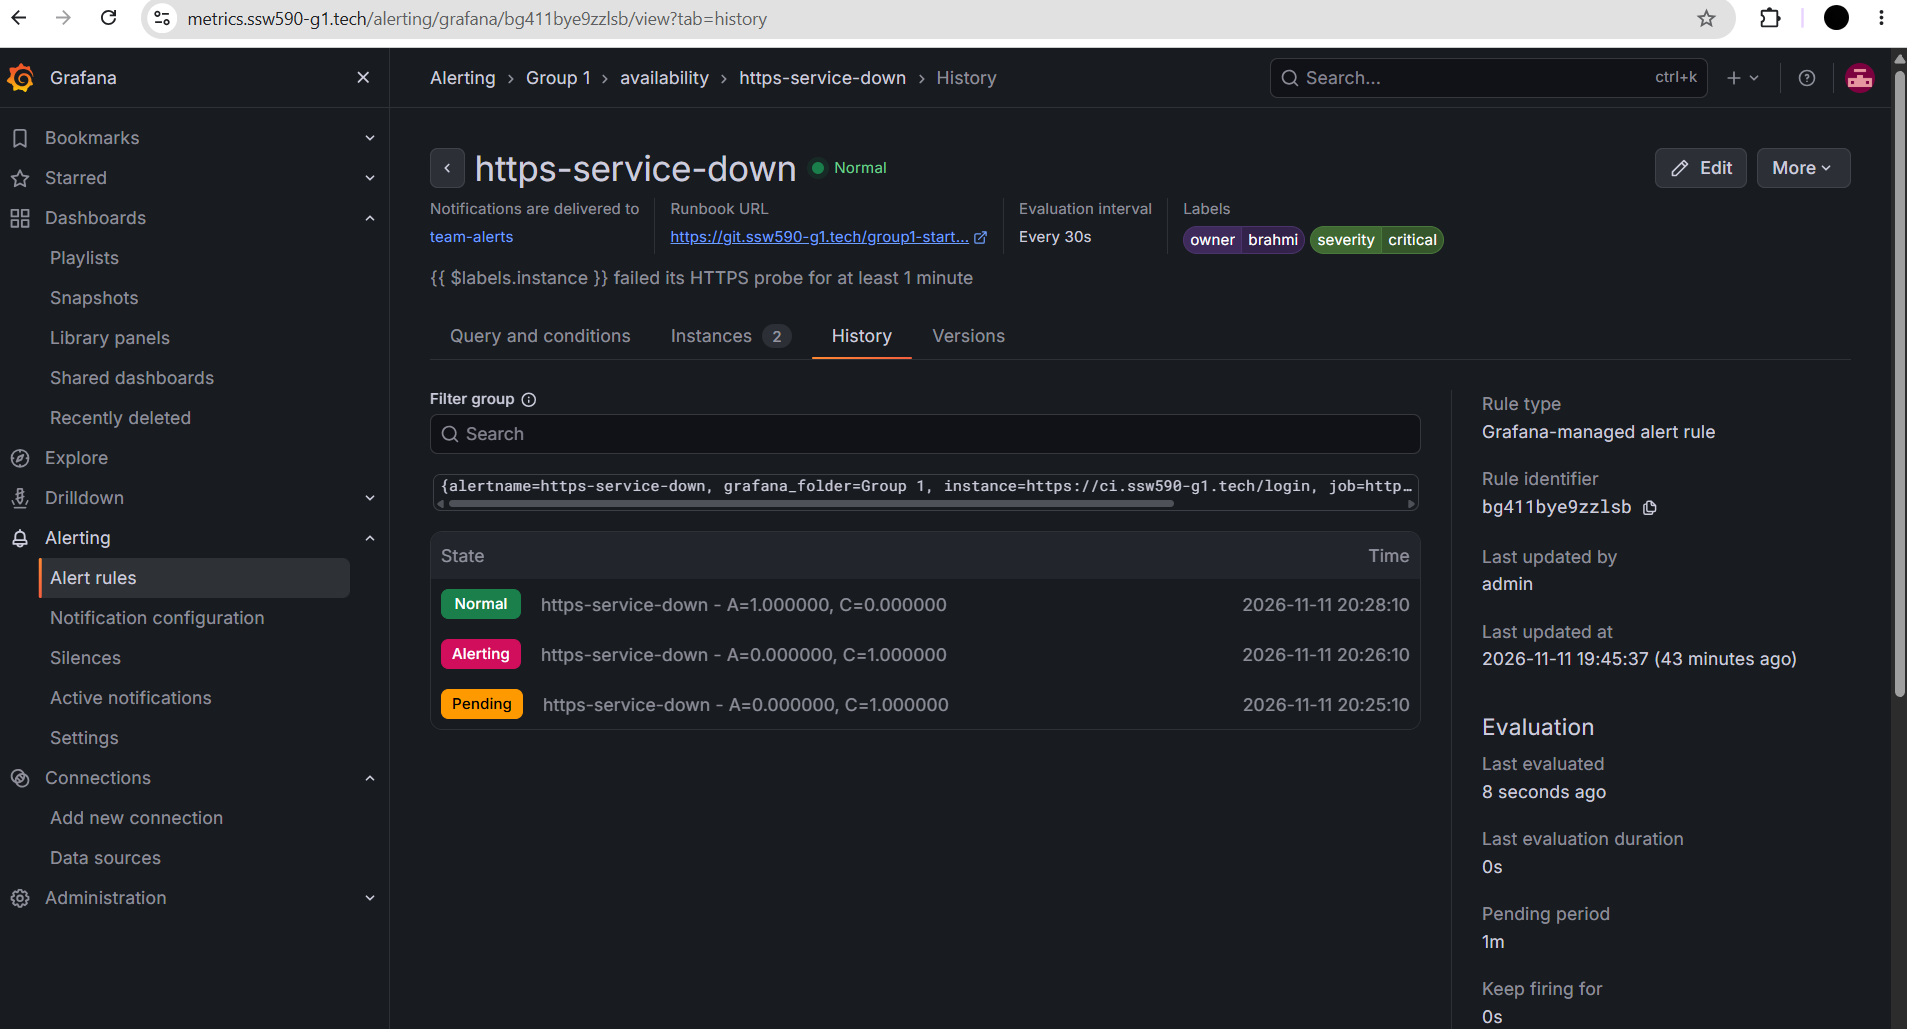
\includegraphics[width=\linewidth]{evidence/163-grafana-jenkins-outage-rule-history-pending-alerting-normal-bd-2026-11-11.png}
\caption{History of the rule for the Jenkins instance: Pending 20:25:10, Alerting 20:26:10, Normal 20:28:10 (EST).}
\label{Fig:E163}
\end{figure}

\begin{figure}[htbp]
\centering
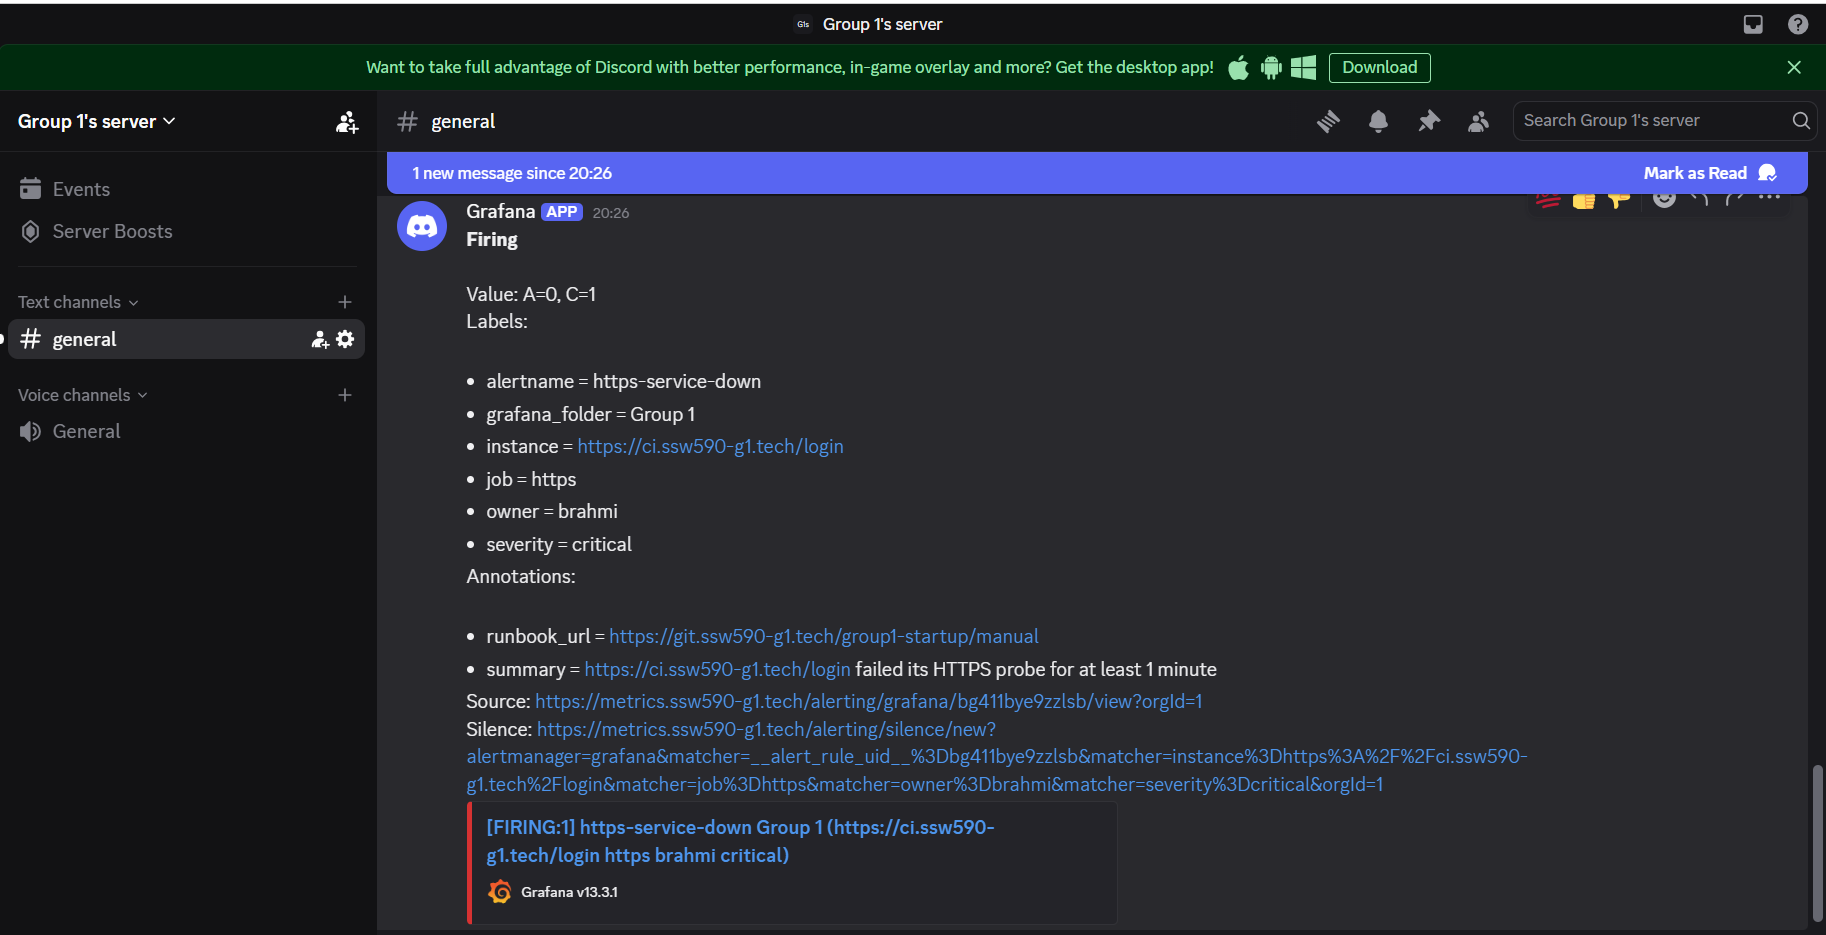
\includegraphics[width=\linewidth]{evidence/164-discord-jenkins-outage-firing-notification-20-26-bd-2026-11-11.png}
\caption{Discord Firing message for \texttt{https://ci.ssw590-g1.tech/login}, 20:26 EST.}
\label{Fig:E164}
\end{figure}

\begin{figure}[htbp]
\centering
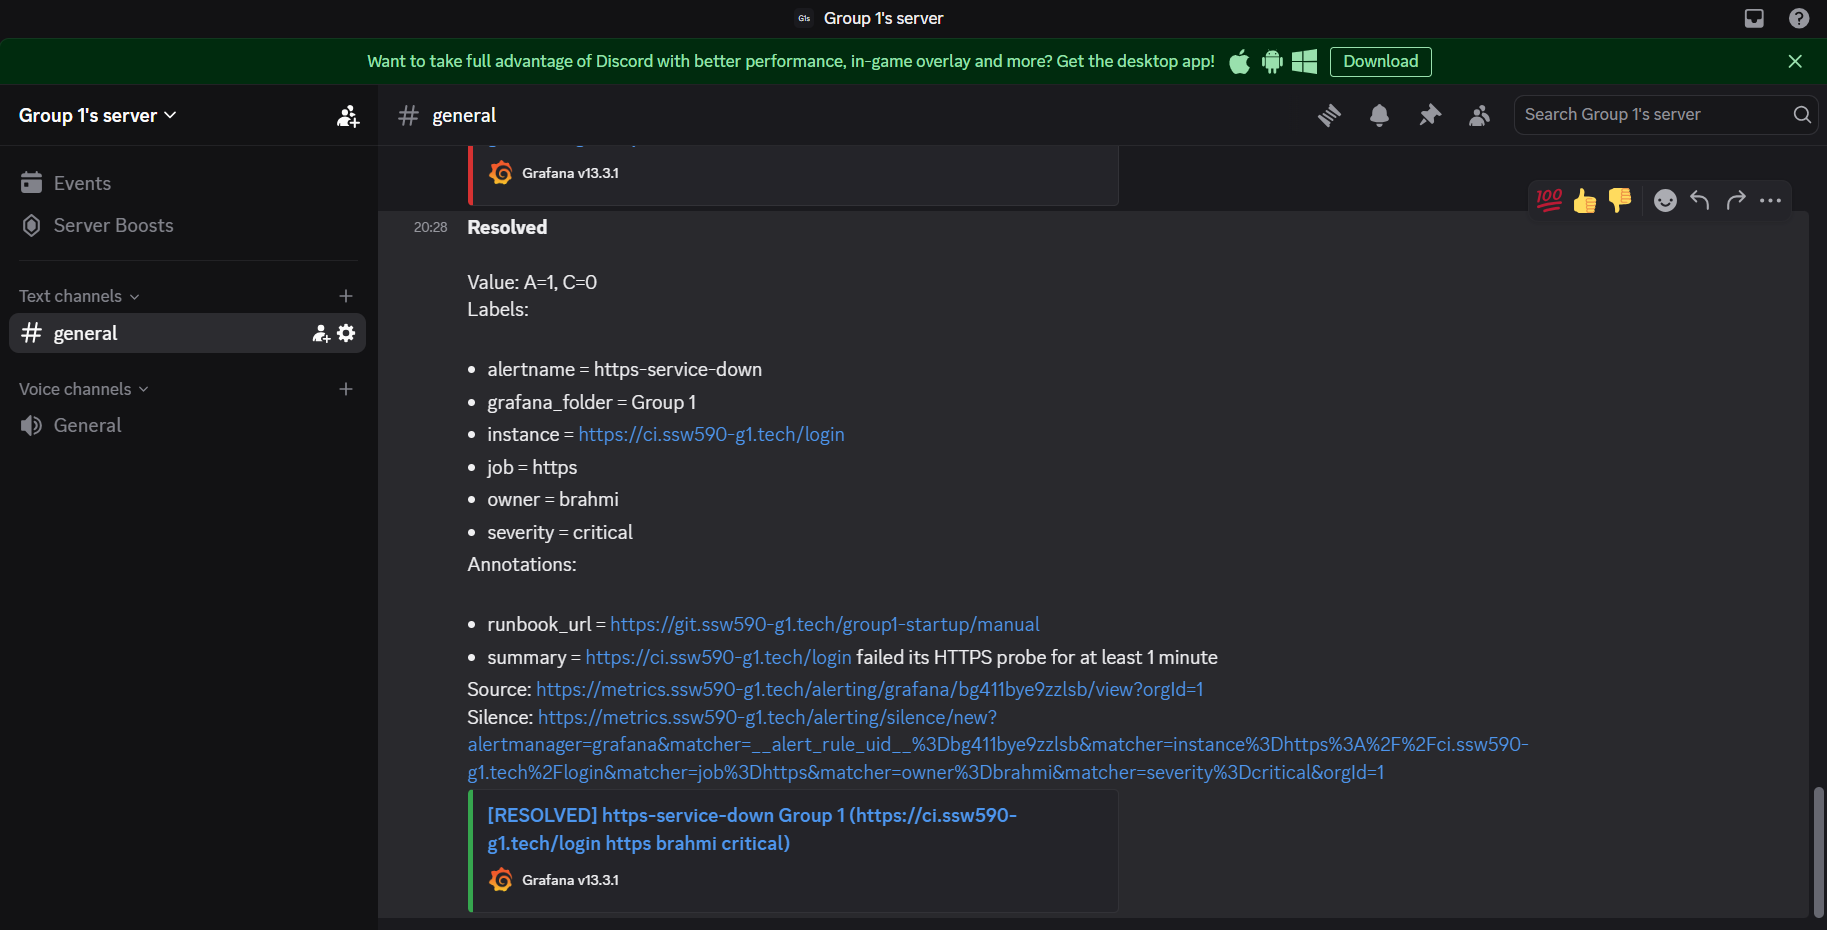
\includegraphics[width=\linewidth]{evidence/165-discord-jenkins-outage-resolved-notification-20-28-bd-2026-11-11.png}
\caption{Discord Resolved message, 20:28 EST.}
\label{Fig:E165}
\end{figure}

\paragraph{Verification.} After the restart, Jenkins' login page answered, a pipeline run of \texttt{main} passed (\FigRef{166}), and the commit status of that run reached Gitea, so the Jenkins-to-Gitea status path works again.
The Prometheus and Grafana restart test followed and is described with the deployment (Section~\ref{Section:sreDeployment}); the record is \ListRef{115}, which also shows the dashboard still present after Grafana's restart (read from Grafana's database, because Grafana 13 keeps dashboards in a new storage table).

\begin{figure}[htbp]
\centering
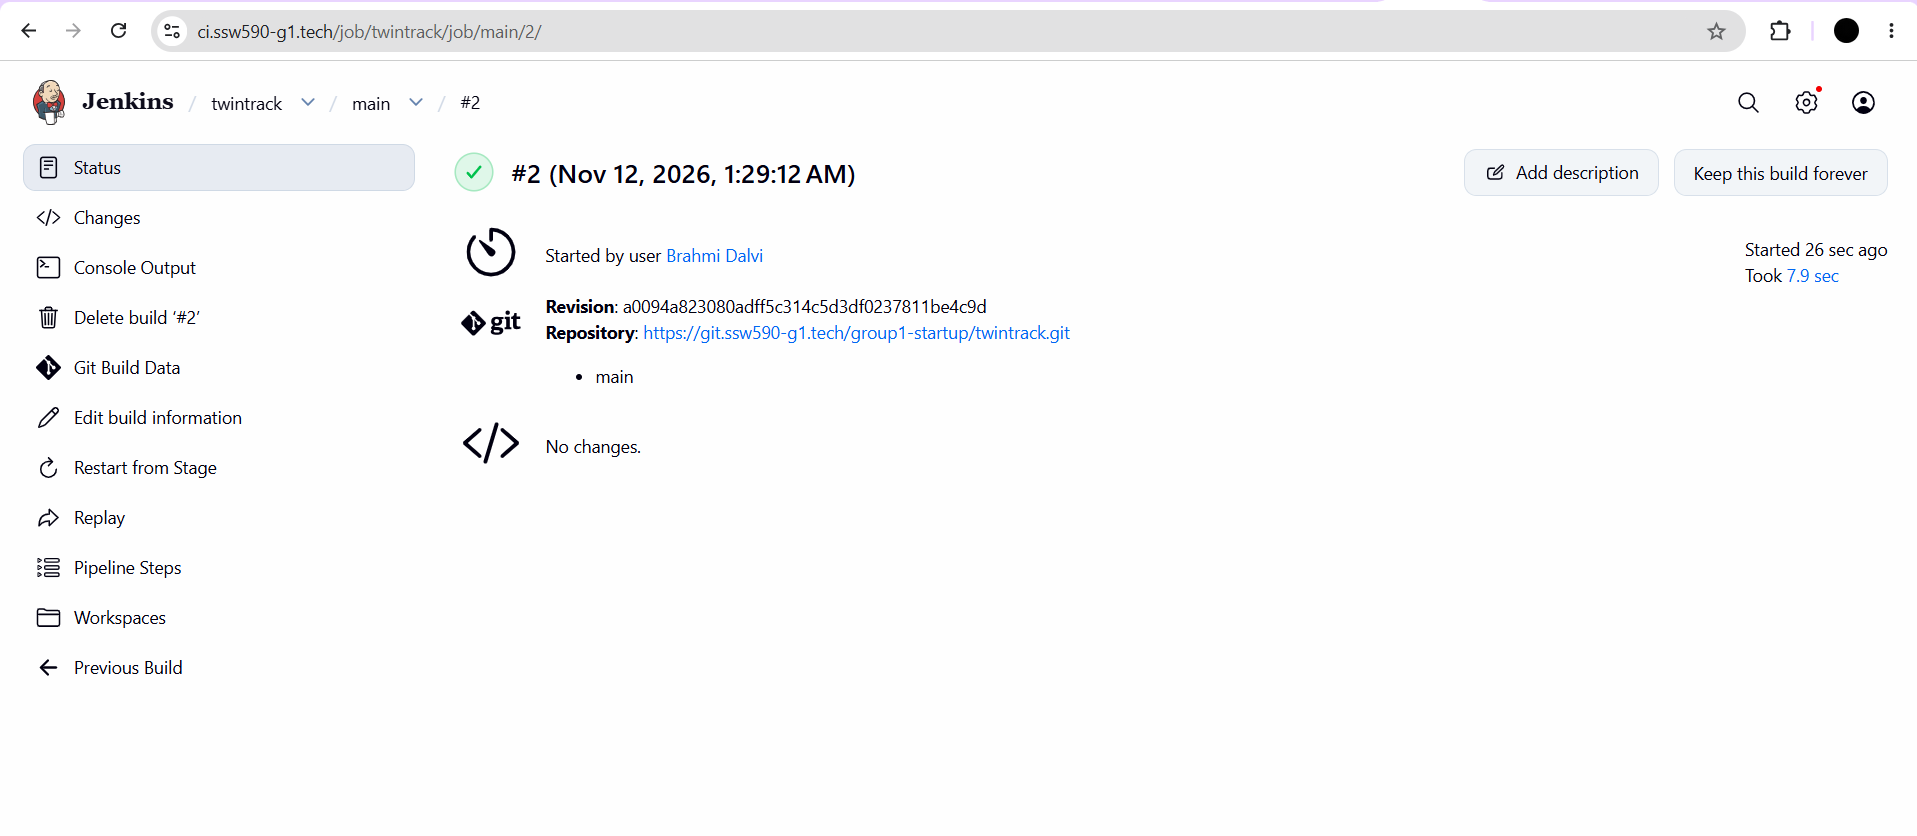
\includegraphics[width=\linewidth]{evidence/166-jenkins-twintrack-main-build-2-success-after-outage-bd-2026-11-11.png}
\caption{Jenkins \texttt{twintrack/main} build \#2 after the outage, Nov 12, 2026, 1:29:12 AM server time (UTC): SUCCESS in 7.9~s.}
\label{Fig:E166}
\end{figure}

\paragraph{Compared with Chapter~4.} In Chapter~\ref{Chapter:Jenkins} a \emph{bad commit} failed its tests and Gitea's merge gate refused the merge, while Jenkins itself was healthy.
Here the commit was fine and the \emph{CI service} was down: nothing failed in Jenkins' tests, no commit status changed, and only monitoring noticed. The two checks cover different failures and neither replaces the other.

\paragraph{Blameless review.} \emph{Impact:} Jenkins was unavailable for 3~min 24~s as seen by the probes (stop to first successful probe); only the team uses it, no build was running, and Gitea stayed up, so nobody lost work.
\emph{Cause:} a deliberate injection, \texttt{docker stop jenkins}, agreed beforehand by BD and SD. \emph{Response:} the rule went Firing after 1~min 45~s, the Discord message arrived about half a minute later, BD restarted Jenkins after reading it, and
Jenkins answered 24~s later; a build and the Gitea status path were checked straight away. \emph{What worked:} the alert fired for the right service only, its summary named the URL, the Resolved message followed 21~s after recovery, and the
numbers matched the configured delays. \emph{What was weak:} the exact acknowledgement time was not written down, the runbook link in the rules is still the manual repository and not a specific page, the one team contact point is a single Discord channel
(if nobody reads it, nothing happens), and the probe that detected the outage runs on the same host as the services.
Measurement gaps: one probe location only, and it runs on the same server, so an outage of the whole host would also stop monitoring; probes every 30~s cannot see shorter outages; the first failing probe time (01:24:49) differs from SD's 15~s polling
(\ListRef{117}) by a few seconds, which is the sampling interval; and the 4~s probe sample in Section~\ref{Section:sreDashboard} was not explained. No person was at fault: the failure was injected on purpose.

\paragraph{Improvement issues.} Two prioritized issues are recorded in the \texttt{infra} repository in Gitea: \textbf{(1) Monitoring shares the monitored server} (owner BD, high priority): add a probe that runs outside this
host, for example a free external uptime check or a scheduled job on another machine, because a failure of the whole instance also stops Prometheus, Grafana, and the alerts. \textbf{(2) Back up the monitoring state and test notifications on a schedule}
(owner SD, medium priority): copy the Grafana and Prometheus volumes off the host and send a monthly test notification, because the restart test shows persistence only, not a backup that can be restored.
They are \href{\GiteaURL/group1-startup/infra/issues/3}{issue \#3} (assigned to BD) and \href{\GiteaURL/group1-startup/infra/issues/4}{issue \#4} (assigned to SD), both open on November 12, 2026.

% ===== BD region: row 8 =====
% Region: sreManual (single owner; edit only your own region)
\section{Manual changes in this version (10 points)}\label{Section:sreManual}
\textbf{Owner:} BD. \textbf{Status:} written November 11, 2026; final scan after the last build \StatusPending.

\paragraph{Version and history.} The manual's version rose from 1.2 to \textbf{1.3} (title page and \ref{Table:DocumentHistory}, the document history): the entry dated November 11, 2026
names the authors (BD, SD, and the AI assistant), lists what changed in this chapter, says that the Hosts and Passwords tables \emph{changed}, and links to \ChapterRef{Sre} and \ChapterRef{HostsPasswords}.

\paragraph{Hosts and Passwords changes.} \textbf{Hosts:} the instance type is \texttt{t3.small} (resized November 10); SSH is allowed from two single addresses, the home address and the campus address (kept for the later assignments;
the campus address is shared by others on that network); the new host \texttt{metrics.ssw590-g1.tech} with Grafana, Prometheus, Node Exporter, and Blackbox Exporter, their versions, memory limits, and private ports (only Grafana reaches Caddy);
the DNS record \texttt{metrics}; the monitoring notes of the Gitea and Jenkins rows. \textbf{Passwords (hints only):} the Grafana administrator (a random first password, then BD's own, set at a prompt on the server), the Grafana user \texttt{sakshi}
(temporary password handed over privately, changed at first sign-in), the Discord webhook URL of the contact point (stored only inside Grafana), the Discord server, and the extended team address list. No secret is written in either table.

\paragraph{Glossary, references, and attribution.} The glossary has new entries for SRE, SLI, SLO, SLA, error budget, Prometheus, Grafana, exporter, and probe. The bibliography has the Chapter~5 sources of the course manual
\cite{GrafanaPromDataSource,GrafanaAlerting,GrafanaDocker,BlackboxExporter,PrometheusInstall,NodeExporter,PrometheusConfig,PrometheusFunctions} and the SRE Workbook chapter on SLOs \cite{GoogleSREWorkbookSLO}; the entries listed as
\emph{not separately opened} were not opened by the authors. Dashboard queries and the Prometheus and Blackbox configuration follow the course manual's examples \cite{DosManual}, adapted to the real URLs; nothing was copied from an imported dashboard.
The AI Prompt Log has the record for this assignment: what the AI assistant did and where it made mistakes, and that no password, token, or webhook URL was ever given to it.

\paragraph{Build and review.} \Todo{link to the successful Gitea Actions run and the reviewed final commit of the manual repository; final scan for TODO and undefined references after the last build}.


